% ============================================================
% 第 1 章  量子力学（续）
% ch01c：原书 p.48–79（PDF 49–80），含 §1.9–§1.12 与本章回顾
% ============================================================

% [原文 p.48]
出乎意料的是，\(E_n\) 恰好对应我们前面求出的无限深方势阱的束缚态能量。在能量 \(E_n\) 上，\(\psi\) 在阱内的波长为
\[
  \frac{2\pi}{\mu}=\frac{2\pi\hbar}{\sqrt{2m(E_n+V_0)}}=\frac{4a}{n+1}.
\]
于是阱宽 \(2a\) 恰好容纳整数个半波长。这一现象称为\emph{共振透射}（resonant transmission）。

我们也可以考虑从右侧入射的波，并寻找如下形式的解
\[
  \psi(x)=
  \begin{cases}
    Be^{-ikx} & x<-a,\\
    C\sin\mu x+D\cos\mu x & -a<x<a,\\
    Fe^{ikx}+Ge^{-ikx} & x>a.
  \end{cases}
\]
\begin{center}
  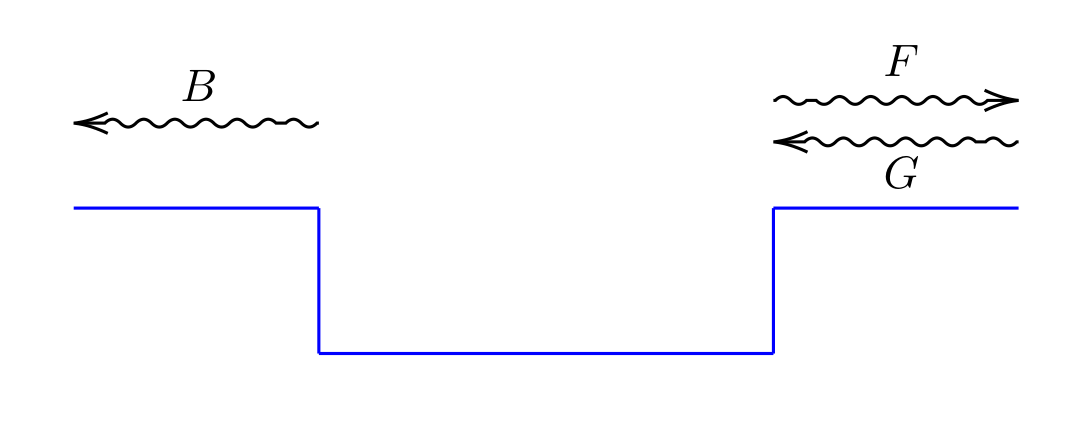
\includegraphics[width=0.66\textwidth]{figures/fig_p49_a.png}
\end{center}
% [图：原书 p.48，图内仅有数学字母标注]

解释方式类似。反射系数与透射系数为
\[
  R=\frac{|F|^2}{|G|^2},\qquad T=\frac{|B|^2}{|G|^2}.
\]
一般地，也可以有从两侧同时入射的波
\[
  \psi(x)=
  \begin{cases}
    Ae^{ikx}+Be^{-ikx} & x<-a,\\
    C\sin\mu x+D\cos\mu x & -a<x<a,\\
    Fe^{ikx}+Ge^{-ikx} & x>a.
  \end{cases}
\]
\begin{center}
  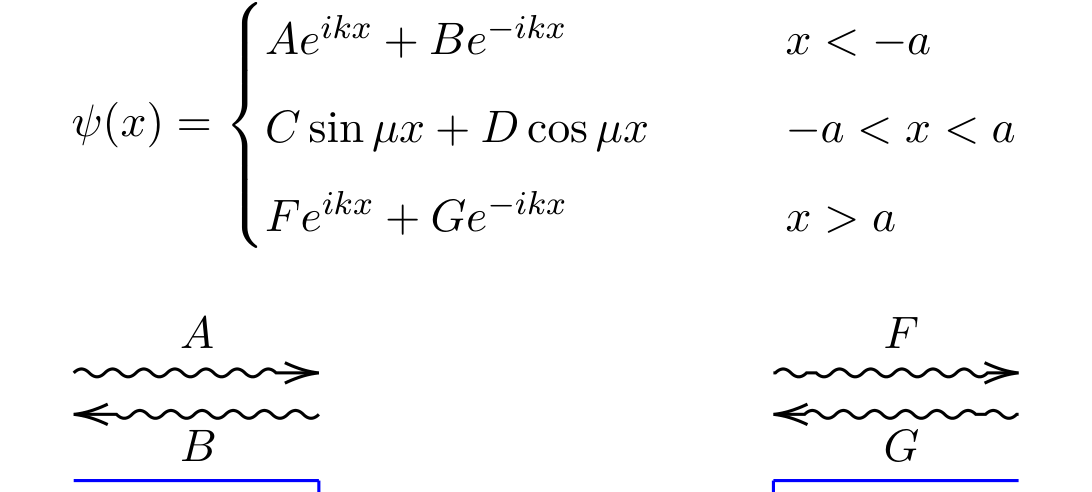
\includegraphics[width=0.66\textwidth]{figures/fig_p49_b.png}
\end{center}
% [图：原书 p.48，图内仅有数学字母标注]

此时 \(A,G\) 表示入射波，\(B,F\) 表示出射波。

\section{散射}

本节以粒子在一维情形下的散射为例，讨论散射过程的基本想法。我们说明它与薛定谔算子的连续谱有何关系。

% [原文 p.49]
\subsection{波包散射}
研究散射问题时，我们考虑从远处飞来、被局域相互作用产生的势散射的粒子。

\begin{center}
\begin{tikzpicture}[scale=0.95,>=Stealth]
  \node[blue] at (-4.05,0) {\small 入射};
  \foreach \y in {0.5,0,-0.5}
    \draw[blue,->] (-3.0,\y)--(-1.5,\y);
  \draw[fill=gray!8] (0,0) circle (1.0);
  \draw[thick] (0,1)--(-1,0);
  \draw[thick] (0.3403,0.9403)--(-0.9403,-0.3403);
  \draw[thick] (0.6,0.8)--(-0.8,-0.6);
  \draw[thick] (0.8,0.6)--(-0.6,-0.8);
  \draw[thick] (0.9403,0.3403)--(-0.3403,-0.9403);
  \draw[thick] (1,0)--(0,-1);
  \draw (0,0) circle (1.0);
  \foreach \a in {32,-28,-152}
    \draw[red,->] (\a:1.12)--(\a:2.55);
  \node[red] at (3.15,-0.12) {\small 出射};
\end{tikzpicture}
\end{center}
% [图：原书 p.49，本图按原文重绘，图内标注已译为中文；原图无题注]

我们考虑一维粒子在紧支势 \(V(x)\) 中的散射，
\[
  V(x)=0\qquad \text{for } |x|\ge R.
\]
\begin{center}
  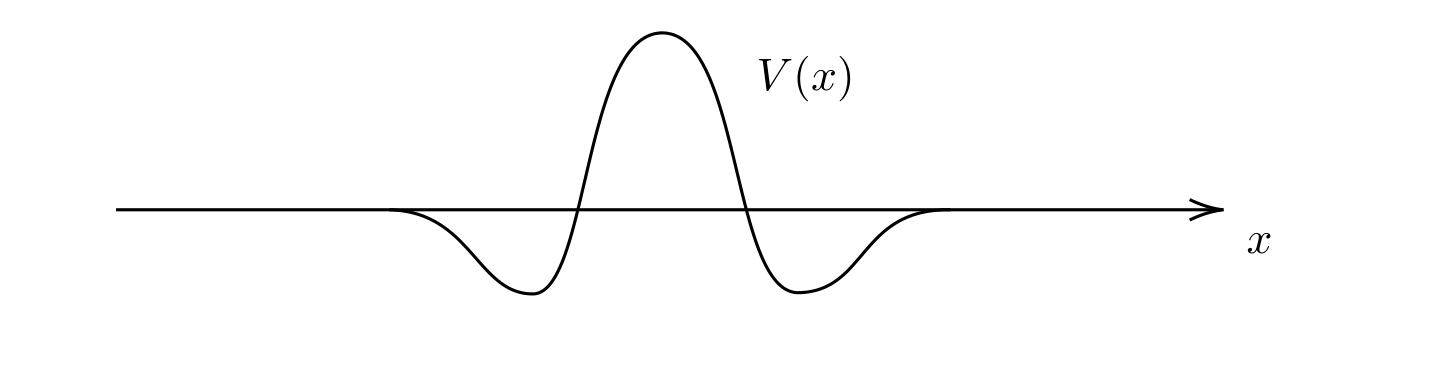
\includegraphics[width=0.62\textwidth]{figures/fig_p50_b.png}
\end{center}
% [图：原书 p.49，图内仅有数学符号标注]

设粒子从 \(x=-\infty\) 处来。按量子力学，这样的粒子由一个波包表示，
\begin{center}
\begin{tikzpicture}[scale=0.95,>=Stealth]
  \draw[->] (-3.9,0)--(3.9,0);
  \draw[thick] plot[domain=-2.55:-0.45,samples=80] (\x,{0.85*exp(-((\x+1.5)/0.26)^2)});
  \draw[->] (-2.05,1.2)--(-1.05,1.2) node[right] {\small $k_0$};
  \node at (-2.05,1.55) {\small 入射};
  \node at (0,-0.62) {\small 相互作用之前};
\end{tikzpicture}
\end{center}
% [图：原书 p.49，本图按原文重绘，图内标注已译为中文；原图无题注]

当粒子进入 \(V\) 的区域后，便与势相互作用。此后它以一定的概率穿过势、朝 \(x=+\infty\) 走去，或者被反射回 \(x=-\infty\)。

\begin{center}
\begin{tikzpicture}[scale=0.95,>=Stealth]
  \draw[->] (-3.9,0)--(3.9,0);
  \draw[thick] plot[domain=-3.1:-1.0,samples=80] (\x,{0.85*exp(-((\x-(-2.05))/0.26)^2)});
  \draw[thick] plot[domain=1.0:3.1,samples=80] (\x,{0.85*exp(-((\x-2.05)/0.26)^2)});
  \draw[->] (-2.05,1.2)--(-3.05,1.2);
  \node at (-2.35,1.55) {\small 反射};
  \draw[->] (2.05,1.2)--(3.05,1.2);
  \node at (2.35,1.55) {\small 透射};
  \node at (0,-0.62) {\small 相互作用之后};
\end{tikzpicture}
\end{center}
% [图：原书 p.49，本图按原文重绘，图内标注已译为中文；原图无题注]

% [原文 p.50]
确切地说，我们把入射的自由粒子写成一个局域波包
\[
  \psi_{\mathrm{in}}(x,t)=\frac{1}{\sqrt{2\pi}}\int_{\R}dk\,\alpha(k)e^{i(kx-\omega(k)t)},
  \qquad \omega(k)=\frac{\hbar k^2}{2m}.
\]
这里 \(\alpha(k)\) 只在 \(k_0>0\) 的某个小邻域内非零，因此波包以群速度 \(\hbar k_0/m\) 向前行进。我们假设
\[
  \int_{\R}dk\,|\alpha(k)|^2=1,
\]
从而波函数是归一的
\[
  \int_{\R}dx\,|\psi_{\mathrm{in}}(x,t)|^2=1.
\]
为描述散射过程，我们注意到薛定谔方程
\[
  i\hbar\frac{\partial}{\partial t}\psi=\left(-\frac{\hbar^2}{2m}\frac{d^2}{dx^2}+V(x)\right)\psi
\]
对 \(\psi\) 是线性的。这一线性性给出如下策略：先寻找在远处为平面波的解，再关于系数 \(\alpha(k)\) 对这些渐近平面波解作叠加，得到散射的物理波函数。

确切地说，我们考虑定态薛定谔方程
\[
  \left(-\frac{\hbar^2}{2m}\frac{d^2}{dx^2}+V(x)\right)\psi=E\psi,
  \qquad \text{其中}\quad E=\frac{(\hbar k)^2}{2m}>0.
\]
在区域 \(|x|\gg 0\) 上，势 \(V(x)=0\)，因此波函数是 \(e^{\pm ikx}\) 的线性组合。我们寻找形如
\[
  \psi_k(x)=
  \begin{cases}
    e^{ikx}+B(k)e^{-ikx} & x\to-\infty,\\
    C(k)e^{ikx} & x\to+\infty
  \end{cases}
\]
的解。
\begin{center}
  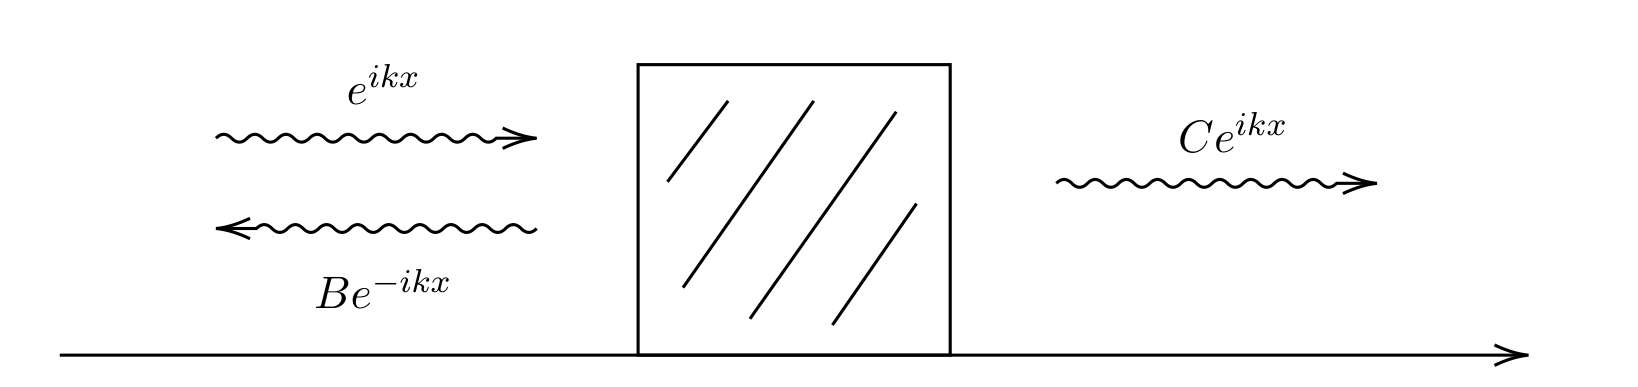
\includegraphics[width=0.72\textwidth]{figures/fig_p51_a.png}
\end{center}
% [图：原书 p.50，图内仅有数学符号标注]

这里 \(B(k),C(k)\) 是依赖于 \(k\) 的常数，由求解定态薛定谔方程定出。这样的解 \(\psi_k\) 不可归一，但落在连续谱中，能量为 \(E_k=\frac{(\hbar k)^2}{2m}\)。

设已求得 \(\psi_k\)。于是由
\[
  \psi(x,t)=\frac{1}{\sqrt{2\pi}}\int_{\R}dk\,\alpha(k)\psi_k(x)e^{-i\frac{\hbar k^2}{2m}t}
\]
得到薛定谔方程的一个解。在区域 \(x\to-\infty\) 上有
\[
  \psi(x,t)=\psi_{\mathrm{in}}(x,t)+\psi_R(x,t),
\]

% [原文 p.51]
其中 \(\psi_{\mathrm{in}}(x,t)\) 是上面准备好的入射波包，而
\[
  \psi_R(x,t)=\frac{1}{\sqrt{2\pi}}\int_{\R}dk\,\alpha(k)B(k)e^{-i\left(kx+\frac{\hbar k^2}{2m}t\right)}
\]
表示反射波包。

在区域 \(x\to+\infty\) 上有
\[
  \psi(x,t)=\frac{1}{\sqrt{2\pi}}\int_{\R}dk\,\alpha(k)C(k)e^{i\left(kx-\frac{\hbar k^2}{2m}t\right)},
\]
它表示透射波包。于是这个波函数 \(\psi(x,t)\) 包含了入射粒子 \(\psi_{\mathrm{in}}\) 与势 \(V(x)\) 散射的量子信息。

\subsection{\(S\) 矩阵}

\(S\) 矩阵即散射矩阵，讲的是散射过程前后粒子态之间的关系。我们在一维散射过程中说明 \(S\) 矩阵。

考虑局域的一维紧支势 \(V(x)\)。如上文所述，散射过程完全由薛定谔方程的解决定，这些解在势垒外 \(|x|\to\pm\infty\) 处是平面波。我们寻找定态薛定谔方程
\[
  \left(-\frac{\hbar^2}{2m}\frac{d^2}{dx^2}+V(x)\right)\psi(x)=E\psi(x),
  \qquad E=\frac{(\hbar k)^2}{2m}
\]
的解，它们具有渐近平面波行为
\[
  \psi(x)=
  \begin{cases}
    Ae^{ikx}+Be^{-ikx} & x\to-\infty,\\
    Ce^{ikx}+De^{-ikx} & x\to+\infty.
  \end{cases}
\]
\begin{center}
  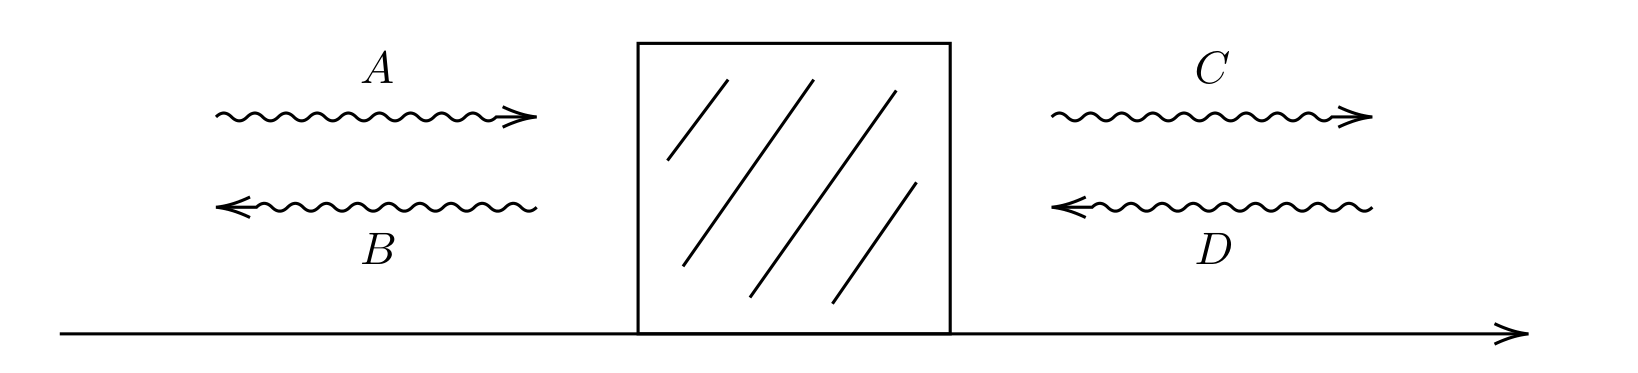
\includegraphics[width=0.72\textwidth]{figures/fig_p52_a.png}
\end{center}
% [图：原书 p.51，图内仅有数学字母标注]

\begin{itemize}[leftmargin=2em,itemsep=1pt]
  \item \(D=0\) 的情形对应振幅为 \(A\) 的波从左侧入射的散射过程。此时 \(C\) 是透射波的振幅，\(B\) 是反射波的振幅。
  \item \(A=0\) 的情形对应振幅为 \(D\) 的波从右侧入射的散射过程。此时 \(B\) 是透射波的振幅，\(C\) 是反射波的振幅。
\end{itemize}

一般地，可以同时有左侧与右侧的入射波。我们把入射波的振幅写成一个列向量
\[
  \Psi_{\mathrm{in}}=\begin{pmatrix}A\\ D\end{pmatrix},
\]

% [原文 p.52]
把出射波的振幅写成列向量
\[
  \Psi_{\mathrm{out}}=\begin{pmatrix}B\\ C\end{pmatrix}.
\]
由于薛定谔方程是线性的，\(\Psi_{\mathrm{out}}\) 与 \(\Psi_{\mathrm{in}}\) 由一个线性关系相联
\[
  \Psi_{\mathrm{out}}=S\Psi_{\mathrm{in}},
\]
即
\[
  \begin{pmatrix}B\\ C\end{pmatrix}
  =\begin{pmatrix}S_{11}&S_{12}\\ S_{21}&S_{22}\end{pmatrix}
  \begin{pmatrix}A\\ D\end{pmatrix}.
\]
起转移作用的矩阵
\[
  S=\begin{pmatrix}S_{11}&S_{12}\\ S_{21}&S_{22}\end{pmatrix}
\]
称为 \(S\) 矩阵。矩阵元 \(S_{ij}\) 是波矢 \(k\) 的函数，这些函数由局域势 \(V(x)\) 完全确定。

为了看清 \(S\) 的矩阵元的含义，取 \(D=0\)，此时
\[
  S\begin{pmatrix}A\\ 0\end{pmatrix}=\begin{pmatrix}S_{11}A\\ S_{21}A\end{pmatrix}.
\]
这说明，对从左侧入射的波，\(S_{11}\) 是反射振幅，\(S_{21}\) 是透射振幅。类似地，取 \(A=0\)
\[
  S\begin{pmatrix}0\\ D\end{pmatrix}=\begin{pmatrix}S_{12}D\\ S_{22}D\end{pmatrix}.
\]
这说明，对从右侧入射的波，\(S_{12}\) 是透射振幅，\(S_{22}\) 是反射振幅。

把透射振幅与反射振幅取模平方，就得到相应的透射系数与反射系数。

\subsection{酉性}

\(S\) 矩阵实际上是酉的。为看清这一点，考虑 \(\psi\) 的概率流
\[
  j(x)=\frac{\hbar}{m}\Imag\left(\bar\psi\frac{d}{dx}\psi\right).
\]
对定态，概率密度 \(\rho=|\psi|^2\) 与时间无关。于是概率的局域守恒（它由 \(\psi\) 的薛定谔方程推出）
\[
  \frac{\partial\rho}{\partial t}+\frac{\partial}{\partial x}j=0
\]
给出 \(\frac{d}{dx}j(x)=0\)。所以 \(j(x)\) 必为常数。

% [原文 p.53]
由 \(\psi(x)\) 的渐近行为得到
\[
  j(x)=
  \begin{cases}
    \frac{\hbar k}{m}\left(|A|^2-|B|^2\right) & x\to-\infty,\\[4pt]
    \frac{\hbar k}{m}\left(|C|^2-|D|^2\right) & x\to+\infty.
  \end{cases}
\]
所以
\[
  |A|^2-|B|^2=|C|^2-|D|^2
  \quad\Longrightarrow\quad
  |A|^2+|D|^2=|B|^2+|C|^2.
\]
换言之，
\[
  \bar\Psi_{\mathrm{out}}^{\,t}\Psi_{\mathrm{out}}=\bar\Psi_{\mathrm{in}}^{\,t}\Psi_{\mathrm{in}}.
\]
因此线性变换 \(S\) 保持厄米内积，即 \(S\) 是酉的
\[
  S^*S=1.
\]
这里 \(S^*:=\bar S^{\,t}\)。

\subsection{时间反演对称性}

设势 \(V=V(x)\) 与时间无关。此时薛定谔方程
\[
  i\hbar\frac{\partial}{\partial t}\psi=\hat H\psi
\]
具有时间反演对称性：若 \(\psi(x,t)\) 是解，则 \(\bar\psi(x,-t)\) 也是解，只是时间方向反了过来。对定态薛定谔方程，若 \(\psi(x)\) 满足
\[
  \left(-\frac{\hbar^2}{2m}\frac{d^2}{dx^2}+V(x)\right)\psi(x)=E\psi(x),
\]
则 \(\bar\psi(x)\) 也给出一个解。

现在给定满足
\[
  \psi(x)=
  \begin{cases}
    Ae^{ikx}+Be^{-ikx} & x\to-\infty,\\
    Ce^{ikx}+De^{-ikx} & x\to+\infty
  \end{cases}
\]
的 \(\psi(x)\)，时间反演后的解 \(\bar\psi(x)\) 满足
\[
  \bar\psi(x)=
  \begin{cases}
    \bar B e^{ikx}+\bar A e^{-ikx} & x\to-\infty,\\
    \bar D e^{ikx}+\bar C e^{-ikx} & x\to+\infty.
  \end{cases}
\]
在这组表示下，\(\bar\Psi_{\mathrm{in}}=\begin{pmatrix}\bar B\\ \bar C\end{pmatrix}\)，\(\bar\Psi_{\mathrm{out}}=\begin{pmatrix}\bar A\\ \bar D\end{pmatrix}\)。因此
\[
  \begin{pmatrix}\bar A\\ \bar D\end{pmatrix}
  =S\begin{pmatrix}\bar B\\ \bar C\end{pmatrix}
  \quad\Longrightarrow\quad
  \begin{pmatrix}B\\ C\end{pmatrix}
  =\bar S^{-1}\begin{pmatrix}A\\ D\end{pmatrix}.
\]
由此可得
\[
  S=\bar S^{-1}
  \quad\stackrel{\text{\(S\) 的酉性}}{\Longrightarrow}\quad
  S=S^t.
\]
所以时间反演对称性蕴含 \(S\) 矩阵是对称的。

\takeaway{一维散射可用波包描述：入射波包被紧支势作用后分成反射与透射两部分。\(S\) 矩阵把入射振幅线性地映为出射振幅，其矩阵元分别是反射振幅与透射振幅。概率流守恒使 \(S\) 酉，时间反演对称性使 \(S\) 对称。}

% [原文 p.54]
\section{WKB 近似}

WKB 方法得名于 Gregor Wentzel、Hendrik Kramers 与 Léon Brillouin，它为系数随空间缓慢变化的线性微分方程提供近似解。在量子力学的应用中，它也称为\emph{半经典近似}（semi-classical approximation）。

\subsection{近似方案}

考虑一维定态薛定谔方程
\[
  \left(-\frac{\hbar^2}{2m}\frac{d^2}{dx^2}+V(x)\right)\psi=E\psi.
\]
我们分三个不同的区域分析解 \(\psi\)。

\medskip
\noindent（1）经典允许区。它对应 \(V(x)<E\) 的位置。经典地，运动能量为
\[
  E=\frac{p^2}{2m}+V(x).
\]
所以经典粒子只能在这一区域运动。

\noindent（2）经典禁区。它对应 \(V(x)>E\) 的位置。经典粒子不能进入这一区域。不过，正如前面对谐振子与方势阱束缚态所见，量子粒子可以以一定的概率穿入这一区域。

\noindent（3）转折点。它对应 \(V(x)=E\) 的位置。

\begin{center}
\begin{tikzpicture}[scale=0.95,>=Stealth]
  \draw[->] (-4.3,0)--(4.3,0) node[right] {\small \(x\)};
  \draw[blue] (-3.9,1.2)--(4.0,1.2) node[right,black] {\small \(E\)};
  \draw[thick,domain=-2.2:2.2,samples=100] plot (\x,{0.5*\x*\x-0.3});
  \node at (2.05,2.45) {\small \(V(x)\)};
  \draw[red,->] (-1.95,2.35)--(-1.6,1.35);
  \draw[red,->] (1.95,2.35)--(1.6,1.35);
  \node[red] at (0,2.55) {\small 转折点};
  \draw[red,dashed] (-1.732,0)--(-1.732,1.2);
  \draw[red,dashed] (1.732,0)--(1.732,1.2);
  \node at (-2.95,-0.45) {\small 经典禁区};
  \node at (0,-0.45) {\small 经典允许区};
  \node at (2.95,-0.45) {\small 经典禁区};
\end{tikzpicture}
\end{center}
% [图：原书 p.54，本图按原文重绘，图内标注已译为中文；原图无题注]

WKB 近似方案寻找如下指数形式的定态波函数解（记号说明：这里的 \(S(x)\) 不是 \(S\) 矩阵）
\[
  \psi(x)=e^{\frac{i}{\hbar}S(x)},\qquad S(x)\in\C.
\]
代入薛定谔方程，
\[
  \left(\frac{\hbar^2}{2m}\frac{d^2}{dx^2}-(E-V(x))\right)e^{\frac{i}{\hbar}S(x)}=0
\]

% [原文 p.55]
\[
  \Longrightarrow\qquad (S'(x))^2-i\hbar S''(x)=2m(E-V(x)).
\]
把 \(\hbar\) 看得很小，这个非线性方程可以按 \(\hbar\) 的阶逐次求解：设
\[
  S(x)=\sum_{n=0}^{\infty}\hbar^n S_n(x).
\]
比较下式两端
\[
  \left(\sum_{n=0}^{\infty}\hbar^n S_n'(x)\right)^2
  -i\hbar\sum_{n=0}^{\infty}\hbar^n S_n''(x)=2m(E-V(x)),
\]
得到
\[
  \left\{
  \begin{array}{l}
    S_0'(x)^2=2m(E-V(x))\\[3pt]
    2S_0'(x)S_1'(x)=iS_0''(x)\\[3pt]
    \qquad\vdots\\[3pt]
    2S_0'(x)S_n'(x)=iS_{n-1}''(x)-\sum_{i=1}^{n-1}S_i'(x)S_{n-i}'(x)\\[3pt]
    \qquad\vdots
  \end{array}
  \right.
\]
半经典近似只求解到 \(\hbar^1\) 阶，忽略 \(\hbar^2\) 及更高阶的项。因此我们寻找
\[
  S(x)=S_0(x)+\hbar S_1(x)+O(\hbar^2).
\]
它可以由上述递推关系解出
\[
  S_0(x)=\pm\int^{x}\sqrt{2m(E-V(y))}\,dy
\]
\[
  S_1(x)=\frac{i}{2}\ln\sqrt{2m(E-V(x))}+C_1
\]
其中 \(C_1\) 是某个常数。因此
\[
  \begin{aligned}
    \psi(x)&=\exp\left(\frac{i}{\hbar}\left(S_0(x)+\hbar S_1(x)+O(\hbar^2)\right)\right)\\
    &\simeq e^{\frac{i}{\hbar}S_0(x)}e^{iS_1(x)}\\
    &=\frac{A}{(2m(E-V(x)))^{\frac{1}{4}}}
      e^{\pm\frac{i}{\hbar}\int^{x}\sqrt{2m(E-V(y))}\,dy}
  \end{aligned}
\]
其中 \(A\) 是某个常数。这两个表达式
\[
  \psi_\pm=\frac{A}{(2m(E-V(x)))^{\frac{1}{4}}}
  e^{\pm\frac{i}{\hbar}\int^{x}\sqrt{2m(E-V(y))}\,dy}
\]
就是 WKB 近似的基本形式。

注意这个 WKB 形式在 \(E=V(x)\) 的转折点处会发散。这说明 WKB 近似在转折点附近并不好。那里需要特别的处理，我们很快就会回到这一点。

% [原文 p.56]
\begin{center}
  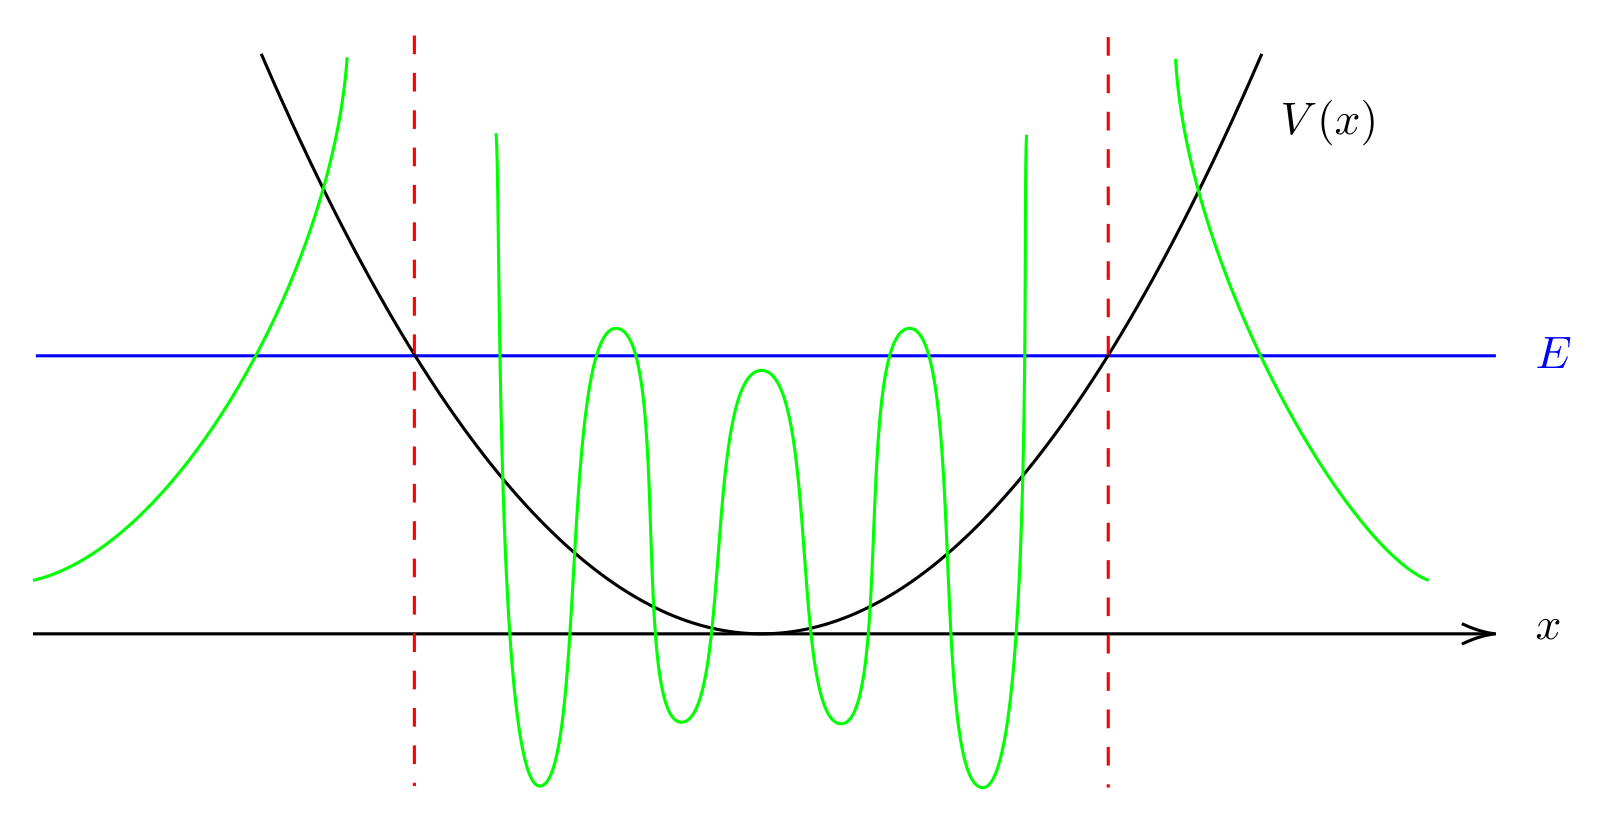
\includegraphics[width=0.72\textwidth]{figures/fig_p57_a.png}
\end{center}
% [图：原书 p.56，图内文字照原样保留]
\fignote{图内文字：WKB approximated solution. Amplitude blows up near the turning points.（译：WKB 近似解。振幅在转折点附近发散。）}

在经典允许区 \(E>V(x)\)，我们写
\[
  E-V(x)=\frac{\hbar^2k(x)^2}{2m}\qquad \text{with}\quad k(x)>0.
\]
此时 WKB 近似解取如下形式（\(A,B\) 是某些常数）
\[
  \psi(x)\simeq\frac{A}{\sqrt{k(x)}}e^{i\int^{x}k(y)dy}
  +\frac{B}{\sqrt{k(x)}}e^{-i\int^{x}k(y)dy}.
\]
带系数 \(A\) 的第一项表示向右运动的波，第二项表示向左运动的波。这个函数在该区域是振荡的。

在经典禁区 \(E<V(x)\)，我们写
\[
  E-V(x)=-\frac{\hbar^2\lambda(x)^2}{2m}\qquad \text{with}\quad \lambda(x)>0.
\]
此时 WKB 近似解取如下形式
\[
  \psi(x)\simeq\frac{A}{\sqrt{\lambda(x)}}e^{\int^{x}\lambda(y)dy}
  +\frac{B}{\sqrt{\lambda(x)}}e^{-\int^{x}\lambda(y)dy}.
\]
这个函数在该区域本质上是指数增长或指数衰减的。

\subsection{转折点与艾里函数}

现在考虑转折点 \(x=a\) 附近的区域。我们寻找一个合适的近似，把这个转折点一侧的振荡型 WKB 近似与另一侧的指数型 WKB 近似连接起来。

\begin{center}
  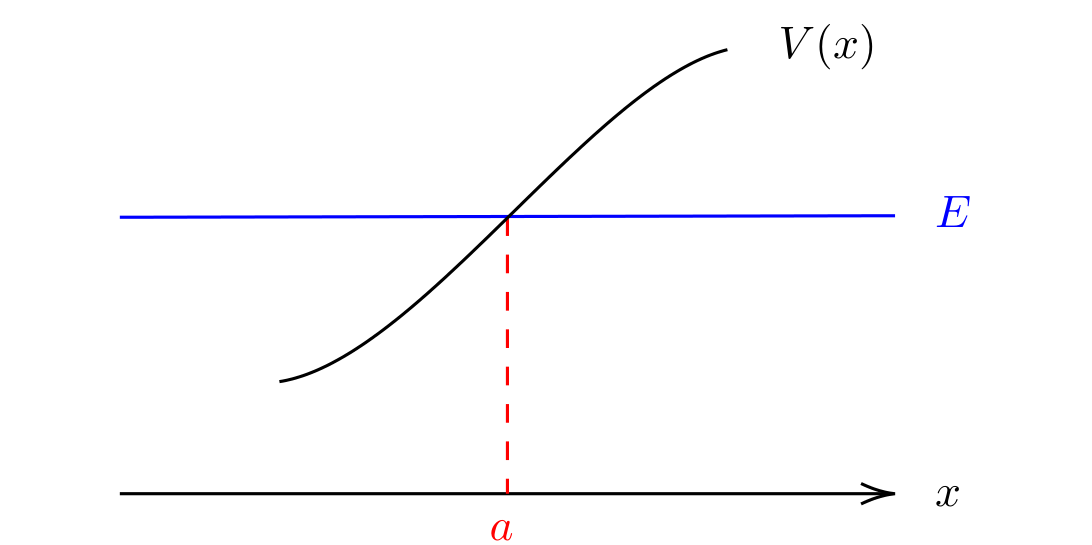
\includegraphics[width=0.46\textwidth]{figures/fig_p57_b.png}
\end{center}
% [图：原书 p.56，图内仅有数学符号标注]

% [原文 p.57]
我们可以在 \(x=a\) 附近用线性函数局部地近似 \(V(x)\)
\[
  V(x)\simeq E+(x-a)V'(a).
\]
由此得到近似方程
\[
  -\frac{\hbar^2}{2m}\frac{d^2}{dx^2}\psi+(x-a)V'(a)\psi=0.
\]
作变量替换
\[
  z=\left(\frac{2mV'(a)}{\hbar^2}\right)^{1/3}(x-a),
\]
上面的近似方程就变为
\[
  \frac{d^2\psi}{dz^2}-z\psi=0.
\]
这就是\emph{艾里方程}（Airy equation）。

艾里方程有两个线性无关的解，记作 \(\mathrm{Ai}(z)\) 与 \(\mathrm{Bi}(z)\)。它们称为\emph{艾里函数}（Airy functions），由下式给出
\[
  \mathrm{Ai}(z)=\frac{1}{\pi}\int_0^{\infty}\cos\left(\frac{t^3}{3}+zt\right)dt
\]
\[
  \mathrm{Bi}(z)=\frac{1}{\pi}\int_0^{\infty}
  \left[\exp\left(-\frac{t^3}{3}+zt\right)+\sin\left(\frac{t^3}{3}+zt\right)\right]dt.
\]
艾里函数 \(\mathrm{Ai}(z),\mathrm{Bi}(z)\) 具有如下近似的渐近行为
\[
  \mathrm{Ai}(z)\simeq
  \begin{cases}
    \dfrac{1}{2\sqrt{\pi}}|z|^{-\frac{1}{4}}\exp\left(-\dfrac{2}{3}|z|^{\frac{3}{2}}\right)
      & z\to+\infty\\[8pt]
    \dfrac{1}{\sqrt{\pi}}|z|^{-\frac{1}{4}}\cos\left(\dfrac{2}{3}|z|^{\frac{3}{2}}-\dfrac{\pi}{4}\right)
      & z\to-\infty
  \end{cases}
\]
\[
  \mathrm{Bi}(z)\simeq
  \begin{cases}
    \dfrac{1}{\sqrt{\pi}}|z|^{-\frac{1}{4}}\exp\left(\dfrac{2}{3}|z|^{\frac{3}{2}}\right)
      & z\to+\infty\\[8pt]
    -\dfrac{1}{\sqrt{\pi}}|z|^{-\frac{1}{4}}\sin\left(\dfrac{2}{3}|z|^{\frac{3}{2}}-\dfrac{\pi}{4}\right)
      & z\to-\infty
  \end{cases}
\]
关键的观察是：这些近似行为恰好把转折点两侧的 WKB 解连接起来。

\subsection{衔接公式}

我们用艾里函数导出转折点 \(x=a\) 附近 WKB 解的衔接条件。

\medskip
\noindent（1）先考虑 \(V'(a)>0\) 的情形。

% [原文 p.58]
\begin{center}
  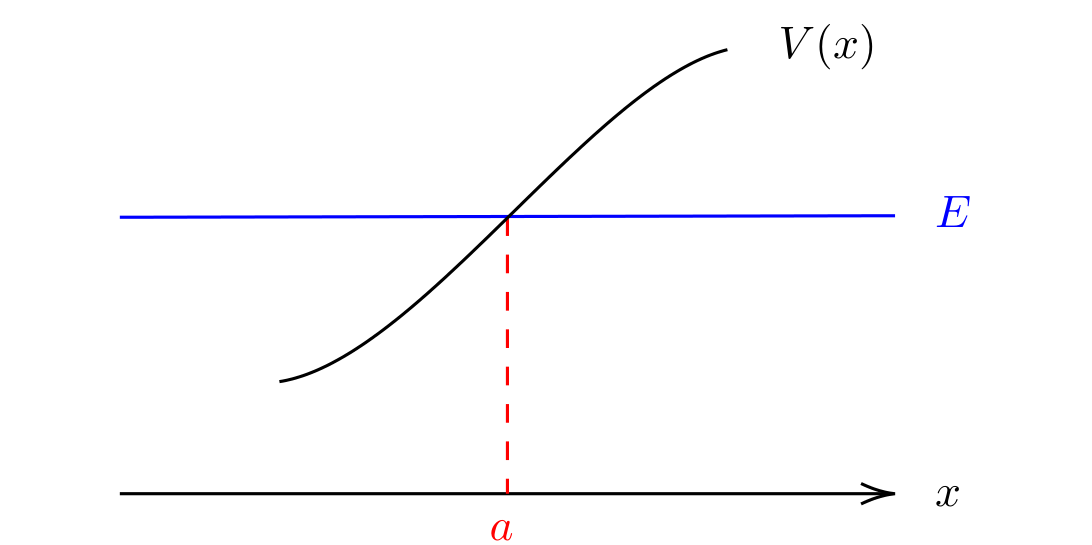
\includegraphics[width=0.46\textwidth]{figures/fig_p57_b.png}
\end{center}
% [图：原书 p.58，图内仅有数学符号标注（与 p.56 的图为同一幅）]

\(V\) 在 \(x=a\) 附近的线性近似为
\[
  V(x)\simeq E+V'(a)(x-a).
\]
在转折点附近的经典允许区 \(x<a\)，近似地有
\[
  k(x)=\frac{\sqrt{2m(E-V(x))}}{\hbar}
  \simeq\left(\frac{2mV'(a)}{\hbar^2}\right)^{1/2}\sqrt{a-x}
\]
以及
\[
  \int_a^x k(y)dy\simeq\left(\frac{2mV'(a)}{\hbar^2}\right)^{1/2}
  \int_a^x\sqrt{a-y}\,dy=-\frac{2}{3}|z|^{3/2}.
\]
在转折点附近的经典禁区 \(x>a\)，近似地有
\[
  \lambda(x)=\frac{\sqrt{2m(V(x)-E)}}{\hbar}
  \simeq\left(\frac{2mV'(a)}{\hbar^2}\right)^{1/2}\sqrt{x-a}
\]
以及
\[
  \int_a^x\lambda(y)dy\simeq\left(\frac{2mV'(a)}{\hbar^2}\right)^{1/2}
  \int_a^x\sqrt{y-a}\,dy=\frac{2}{3}|z|^{3/2}.
\]
设在经典禁区内波函数的主导行为是指数衰减，则 WKB 解必须取如下形式
\[
  \psi(x)\simeq\frac{A}{\sqrt{\lambda(x)}}
  \exp\left(-\int_a^x\lambda(y)dy\right),\qquad x>a.
\]
换言之，指数增长项 \(\frac{1}{\sqrt{\lambda(x)}}\exp\left(\int_a^x\lambda(y)dy\right)\) 不能出现。

\begin{remark}{1.10.1}
  注意，若 \(\psi(x)\) 的主导行为是指数增长，我们就不能排除指数衰减项的出现，因为它被指数增长项压住，在主导行为里看不出来。
\end{remark}

与艾里函数的主导行为比较可知，它只能由 \(\mathrm{Ai}(z)\) 衔接，并且
\[
  \psi(x)\simeq\frac{2A}{\sqrt{k(x)}}
  \cos\left(\int_x^a k(y)dy-\frac{\pi}{4}\right),\qquad x<a.
\]
类似地，若在转折点左侧找到近似波函数
\[
  \psi(x)\simeq\frac{B}{\sqrt{k(x)}}
  \sin\left(\int_x^a k(y)dy-\frac{\pi}{4}\right),\qquad x<a
\]

% [原文 p.59]
则 \(\mathrm{Bi}(z)\) 的主导行为给出
\[
  \psi(x)\simeq-\frac{B}{\sqrt{\lambda(x)}}
  \exp\left(\int_a^x\lambda(y)dy\right).
\]
总结起来，我们得到 \(V'(a)>0\) 时转折点 \(x=a\) 附近 WKB 解的如下衔接条件。

\begin{center}
  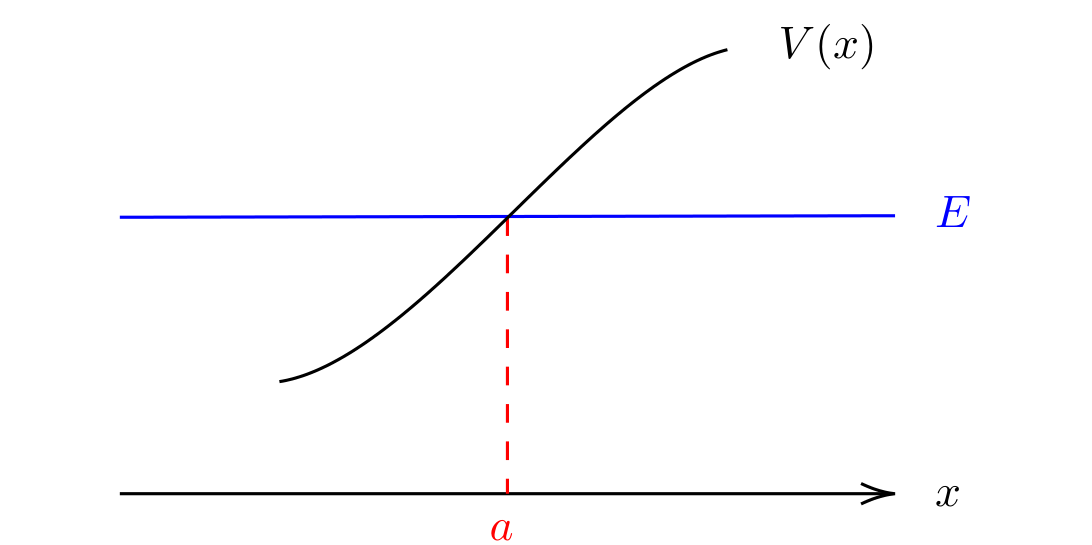
\includegraphics[width=0.46\textwidth]{figures/fig_p57_b.png}
\end{center}
% [图：原书 p.59，图内仅有数学符号标注（与 p.56 的图为同一幅）]

\[
  \frac{2A}{\sqrt{k(x)}}\cos\left(\int_x^a k(y)dy-\frac{\pi}{4}\right)
  \qquad\Longleftarrow\qquad
  \frac{A}{\sqrt{\lambda(x)}}\exp\left(-\int_a^x\lambda(y)dy\right)
\]
\[
  \frac{B}{\sqrt{k(x)}}\sin\left(\int_x^a k(y)dy-\frac{\pi}{4}\right)
  \qquad\Longrightarrow\qquad
  -\frac{B}{\sqrt{\lambda(x)}}\exp\left(\int_a^x\lambda(y)dy\right)
\]
箭头表示推出方向。

\medskip
\noindent（2）再考虑 \(V'(a)<0\) 的情形。讨论类似，我们得到转折点附近 WKB 解的衔接条件。

\begin{center}
  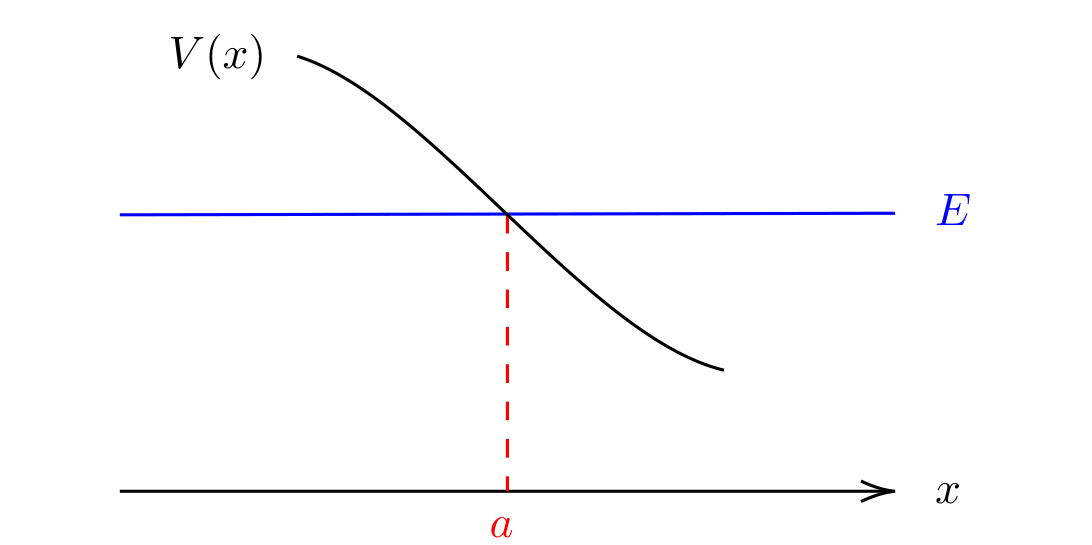
\includegraphics[width=0.46\textwidth]{figures/fig_p60_b.png}
\end{center}
% [图：原书 p.59，图内仅有数学符号标注]

\[
  \frac{A}{\sqrt{\lambda(x)}}\exp\left(-\int_x^a\lambda(y)dy\right)
  \qquad\Longrightarrow\qquad
  \frac{2A}{\sqrt{k(x)}}\cos\left(\int_a^x k(y)dy-\frac{\pi}{4}\right)
\]
\[
  -\frac{B}{\sqrt{\lambda(x)}}\exp\left(\int_x^a\lambda(y)dy\right)
  \qquad\Longleftarrow\qquad
  \frac{B}{\sqrt{k(x)}}\sin\left(\int_a^x k(y)dy-\frac{\pi}{4}\right)
\]

\subsection{半经典量子化规则}

考虑满足
\[
  V(x)\to\infty\qquad \text{as}\quad x\to\pm\infty
\]
的势 \(V(x)\)。

% [原文 p.60]
我们寻找能量为 \(E\) 的束缚态。由谐振子的经验，可以期望允许的能量是离散的。

再设恰有两个转折点 \(x=a\) 与 \(x=b\)，且 \(a<b\)。

\begin{center}
  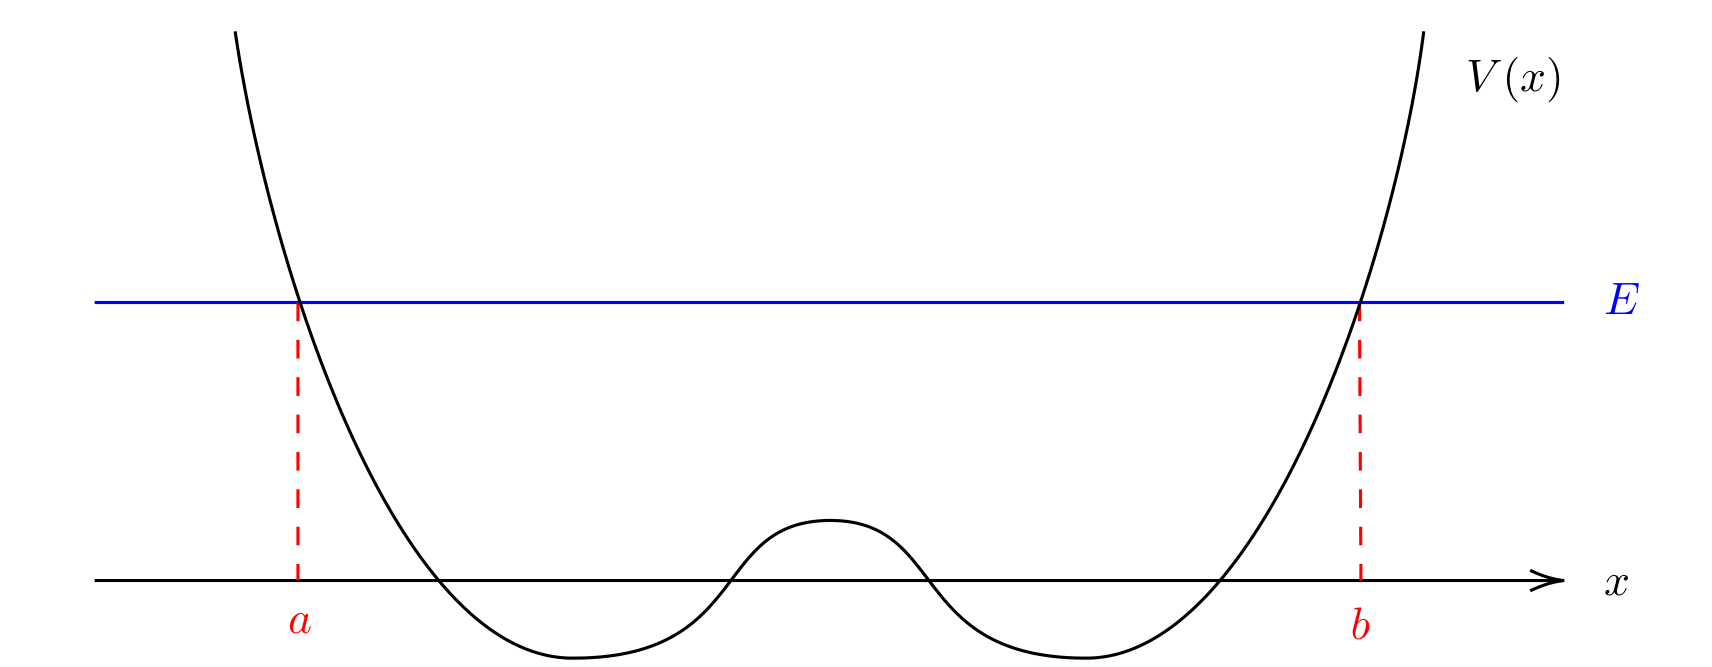
\includegraphics[width=0.72\textwidth]{figures/fig_p61_a.png}
\end{center}
% [图：原书 p.60，图内仅有数学符号标注]

对可归一的束缚态 \(\psi(x)\)，它在禁区内应随 \(x\to\pm\infty\) 衰减。于是 WKB 近似取如下形式
\[
  \psi(x)=
  \begin{cases}
    \dfrac{A}{\sqrt{\lambda(x)}}\exp\left(-\displaystyle\int_a^x\lambda(y)dy\right) & x<a\\[12pt]
    \dfrac{B}{\sqrt{\lambda(x)}}\exp\left(-\displaystyle\int_b^x\lambda(y)dy\right) & x>b
  \end{cases}
\]
由衔接公式，这两个行为都决定了中间经典允许区内的行为。于是自洽条件给出
\[
  \int_a^x k(y)dy-\frac{\pi}{4}
  =-\left(\int_x^b k(y)dy-\frac{\pi}{4}\right)+n\pi
\]
\[
  \Longrightarrow\qquad
  \int_a^b k(y)dy=\pi\left(n+\frac{1}{2}\right)
  \qquad \text{for}\quad n\in\Z.
\]
这称为\emph{爱因斯坦–布里渊–凯勒}（Einstein–Brillouin–Keller，EBK）半经典量子化条件（或\emph{凯勒–马斯洛夫}量子化条件），它通过马斯洛夫指数修正（这里为 \(\frac{1}{2}\)）改进了\emph{玻尔–索末菲}量子化条件。

\begin{example}{1.10.2}
  作为例子，我们考虑谐振子，其势为
  \[
    V(x)=\frac{1}{2}m\omega^2x^2.
  \]
\end{example}

% [原文 p.61]
\begin{center}
  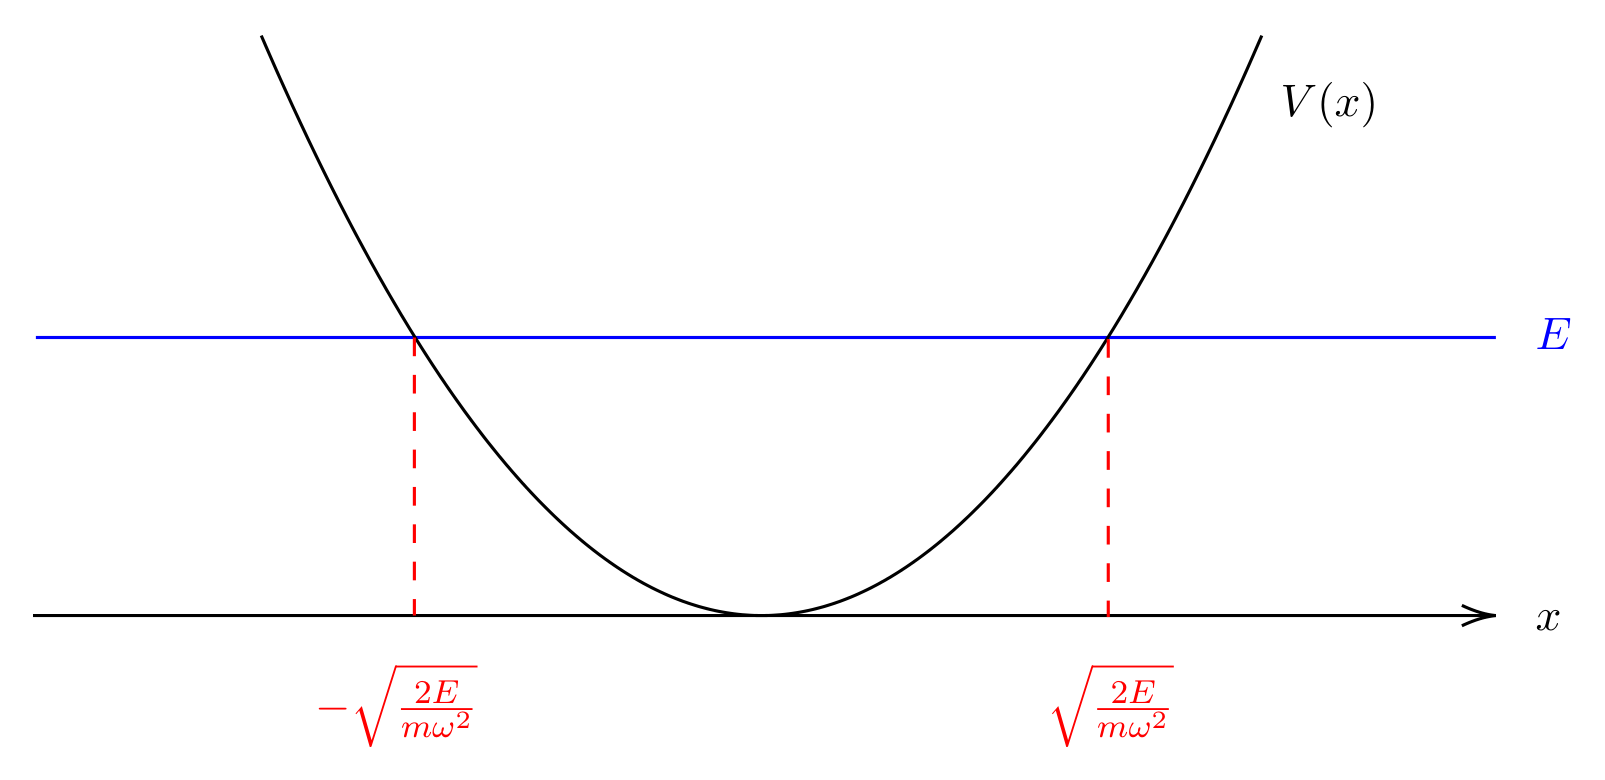
\includegraphics[width=0.72\textwidth]{figures/fig_p62_a.png}
\end{center}
% [图：原书 p.61，图内仅有数学符号标注]

EBK 半经典量子化条件要求
\[
  \frac{\sqrt{2m}}{\hbar}
  \int_{-\sqrt{\frac{2E}{m\omega^2}}}^{\sqrt{\frac{2E}{m\omega^2}}}
  \sqrt{E-\frac{1}{2}m\omega^2x^2}\,dx
  =\pi\left(n+\frac{1}{2}\right)
  \qquad\Longrightarrow\qquad
  E=\left(n+\frac{1}{2}\right)\hbar\omega.
\]
这正是我们前面求出的谐振子的允许能量。

\subsection{量子隧穿}

考虑能量为 \(E\) 的粒子在势 \(V(x)\) 中运动。经典地，粒子只能在 \(V(x)\le E\) 的区域运动。按量子力学，粒子有机会穿过经典上禁止的势垒。这一现象称为\emph{量子隧穿}（quantum tunneling）。

\begin{center}
  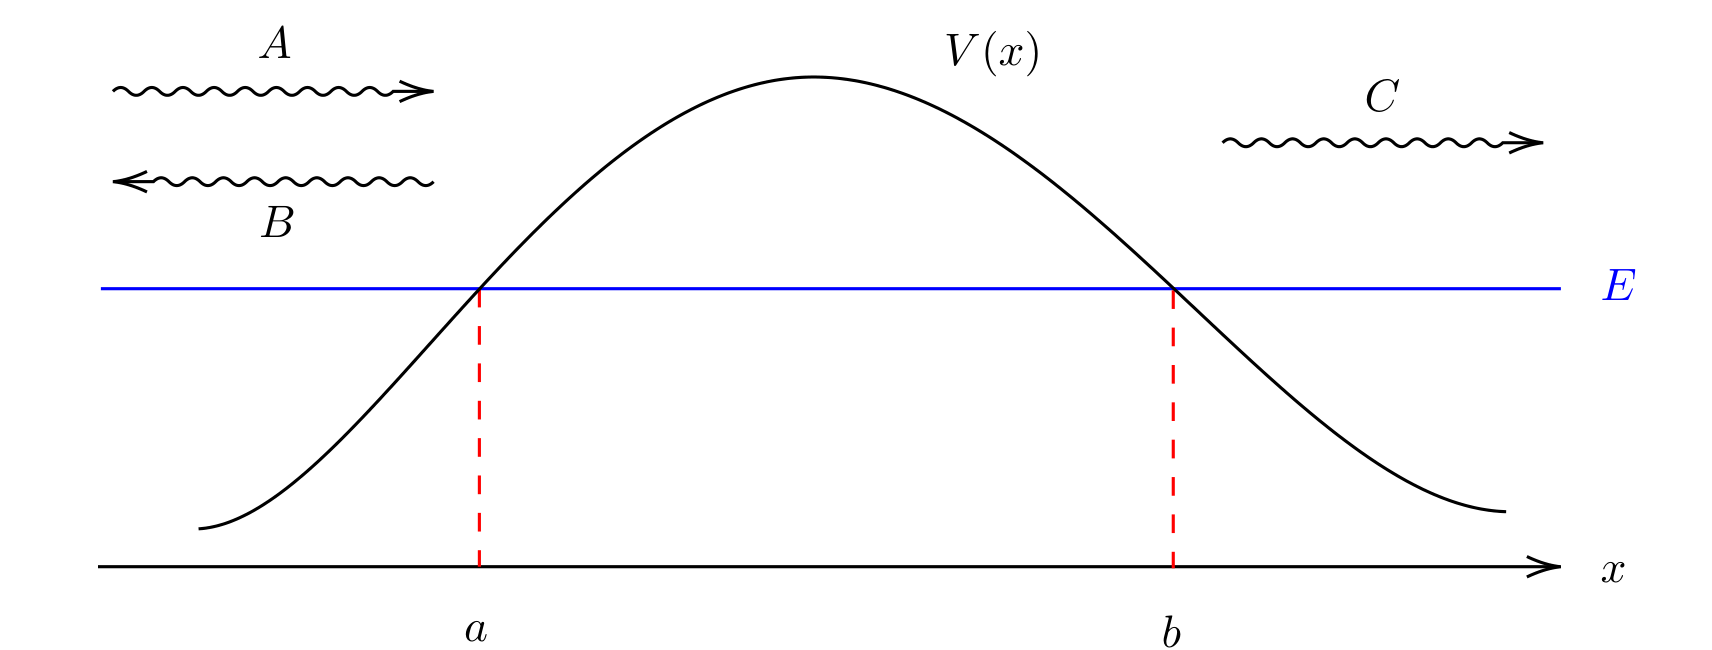
\includegraphics[width=0.72\textwidth]{figures/fig_p62_b.png}
\end{center}
% [图：原书 p.61，图内仅有数学符号标注]

考虑如上势，并设 \(x\to\pm\infty\) 时 \(V(x)\to0\)。设能量 \(E>0\) 且小于势的高度。我们考虑波从左侧入射的散射问题。按量子力学，它有机会穿过势垒。隧穿概率就是我们曾在 §1.8.3 讨论过的透射系数 \(T\)。下面用 WKB 方法给出 \(T\) 的一个近似公式。

把透射波的 WKB 解写成
\[
  \begin{aligned}
    \psi(x)&\simeq\frac{C}{\sqrt{k(x)}}
      \exp\left(i\int_b^x k(y)dy-\frac{\pi}{4}i\right),\qquad x\gg b\\
    &=\frac{C}{\sqrt{k(x)}}\cos\left(\int_b^x k(y)dy-\frac{\pi}{4}\right)
      +\frac{iC}{\sqrt{k(x)}}\sin\left(\int_b^x k(y)dy-\frac{\pi}{4}\right).
  \end{aligned}
\]

% [原文 p.62]
由衔接公式，第二项将衔接到一个在我们从 \(x=b\) 向左移动时指数增长的指数函数
\[
  -\frac{iC}{\sqrt{\lambda(x)}}\exp\left(\int_x^b\lambda(y)dy\right)
  \qquad a<x<b
\]
\[
  =-\frac{iC}{\sqrt{\lambda(x)}}
  \exp\left(-\int_a^x\lambda(y)dy\right)
  \exp\left(\int_a^b\lambda(y)dy\right).
\]
它又将在 \(x=a\) 左侧衔接到
\[
  -\frac{2iC}{\sqrt{k(x)}}\exp\left(\int_a^b\lambda(y)dy\right)
  \cos\left(\int_x^a k(y)dy-\frac{\pi}{4}\right).
\]
把它分解为左行波与右行波，右行波对应的分量为
\[
  -\frac{iC}{\sqrt{k(x)}}\exp\left(\int_a^b\lambda(y)dy\right)
  \exp\left(-i\int_x^a k(y)dy+\frac{\pi}{4}i\right).
\]
这给出近似关系
\[
  |A|=|C|\exp\left(\int_a^b\lambda(y)dy\right).
\]
WKB 近似的透射系数为
\[
  T\simeq\frac{|C|^2}{|A|^2}
  =\exp\left(-2\int_a^b\lambda(y)dy\right)
  =\exp\left(-\frac{2}{\hbar}\int_a^b\sqrt{2m(V(x)-E)}\,dx\right).
\]

\begin{remark}{1.10.3}
  我们将在 §2.7.3 用路径积分方法重新得到这个透射系数的 WKB 公式。在那里，量子隧穿由虚时间中的一条路径实现。
\end{remark}

\begin{example}{1.10.4}
  考虑方势垒的势
  \[
    V(x)=
    \begin{cases}
      V_0 & |x|<a\\
      0   & \text{else}
    \end{cases}
  \]
\end{example}

\begin{center}
  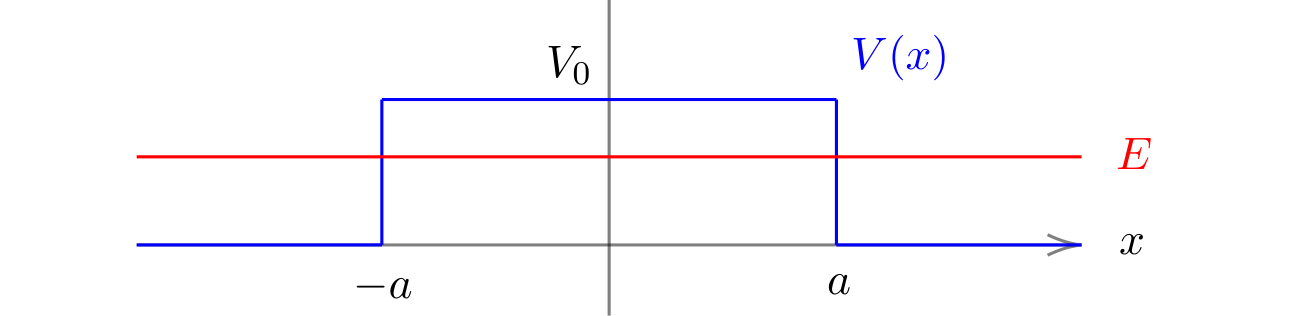
\includegraphics[width=0.60\textwidth]{figures/fig_p63_a.png}
\end{center}
% [图：原书 p.62，图内仅有数学符号标注]

WKB 近似的透射系数为
\[
  T\simeq\exp\left(-\frac{2}{\hbar}\int_{-a}^{a}\sqrt{2m(V(x)-E)}\,dx\right)
  =\exp\left(-\frac{4a}{\hbar}\sqrt{2m(V_0-E)}\right).
\]

\takeaway{WKB 近似把波函数写成指数形式，并按 \(\hbar\) 逐阶展开。允许区内的解是振荡的，禁区内的解是指数型的；转折点附近用艾里函数衔接，得到两侧解的衔接公式。衔接的自洽条件给出 EBK 量子化条件，隧穿概率也由此估算。}

% [原文 p.63]
\section{量子开普勒问题}

本节研究 \(\R^3\) 中处在如下形式势场里的量子粒子
\[
  V(\vec r)=-\frac{Z}{r},\qquad Z>0 \text{ 为常数}.
\]
这里 \(\vec r=(x_1,x_2,x_3)\) 是 \(\R^3\) 上的线性坐标，
\[
  r=\sqrt{x_1^2+x_2^2+x_3^2}
\]
是 \(\vec r\) 的长度。相应的力为
\[
  \vec F=-\nabla V=-\frac{Z}{r^2}\frac{\vec r}{r}.
\]
在我们的假设 \(Z>0\) 下，这个力按平方反比律吸引。例如万有引力与吸引的静电力都属于这一类。平方反比律的问题通常称为\emph{开普勒问题}（Kepler problem）。

经典地，开普勒问题展现出丰富的对称性，并且完全可积。在量子情形，我们将看到束缚态的谱也可以借助对称性精确解出。作为应用，这使我们能计算氢原子的谱。

\subsection{角动量}

\(\R^3\) 中经典粒子运动的角动量为
\[
  \vec J=\vec r\times\vec p
\]
其中 \(\vec p\) 是经典动量。按分量写，
\[
  J_i=\sum_{j,k}\epsilon_{ijk}x_jp_k
  \quad\text{即}\quad
  \begin{cases}
    J_1=x_2p_3-x_3p_2\\
    J_2=x_3p_1-x_1p_3\\
    J_3=x_1p_2-x_2p_1
  \end{cases}
\]
这里 \(\epsilon_{ijk}\) 是 Levi-Civita 符号，\(\epsilon_{123}=1\)。它们的泊松括号关系为
\[
  \{J_i,J_j\}=\sum_{k}\epsilon_{ijk}J_k.
\]
在量子情形，角动量成为自伴算子
\[
  \hat J_i=\sum_{j,k}\epsilon_{ijk}\hat x_j\hat p_k
  \quad\text{即}\quad
  \begin{cases}
    \hat J_1=\hat x_2\hat p_3-\hat x_3\hat p_2\\
    \hat J_2=\hat x_3\hat p_1-\hat x_1\hat p_3\\
    \hat J_3=\hat x_1\hat p_2-\hat x_2\hat p_1
  \end{cases}
\]
正则对易关系
\[
  [\hat x_k,\hat p_j]=i\hbar\delta_{kj}
\]

% [原文 p.64]
给出
\[
  [\hat J_k,\hat J_j]=i\hbar\sum_m\epsilon_{kjm}\hat J_m
\]
\[
  [\hat J_k,\hat x_j]=i\hbar\sum_m\epsilon_{kjm}\hat x_m
\]
\[
  [\hat J_k,\hat p_j]=i\hbar\sum_m\epsilon_{kjm}\hat p_m
\]
从几何上看，这些算子作用在希尔伯特空间 \(L^2(\R^3)\) 上，其中 \(p_k=-i\hbar\frac{\partial}{\partial x_k}\)。于是
\[
  \begin{cases}
    \dfrac{i}{\hbar}\hat J_1=x_2\dfrac{\partial}{\partial x_3}-x_3\dfrac{\partial}{\partial x_2}\\[8pt]
    \dfrac{i}{\hbar}\hat J_2=x_3\dfrac{\partial}{\partial x_1}-x_1\dfrac{\partial}{\partial x_3}\\[8pt]
    \dfrac{i}{\hbar}\hat J_3=x_1\dfrac{\partial}{\partial x_2}-x_2\dfrac{\partial}{\partial x_1}
  \end{cases}
\]
它们分别生成 \(x_2x_3\) 平面、\(x_3x_1\) 平面、\(x_1x_2\) 平面中的旋转。令
\[
  \hat J^2:=\hat J\cdot\hat J=\hat J_1^2+\hat J_2^2+\hat J_3^2.
\]
直接验证可知，\(\hat J^2\) 与 \(\hat J_1,\hat J_2,\hat J_3\) 对易
\[
  [\hat J^2,\hat J_1]=[\hat J^2,\hat J_2]=[\hat J^2,\hat J_3]=0.
\]
\(\hat J^2\) 称为\emph{卡西米尔元}（Casimir element）。

开普勒问题的哈密顿算子
\[
  \hat H=\frac{\hat p^2}{2m}-\frac{Z}{r}
\]
显然是旋转不变的。因此
\[
  [\hat H,\hat J_k]=0,\qquad k=1,2,3.
\]
这也可以直接验证。

我们关心束缚态，即定态薛定谔方程的可归一的解。此时这种束缚态的能量 \(E\) 必须为负。

\begin{center}
  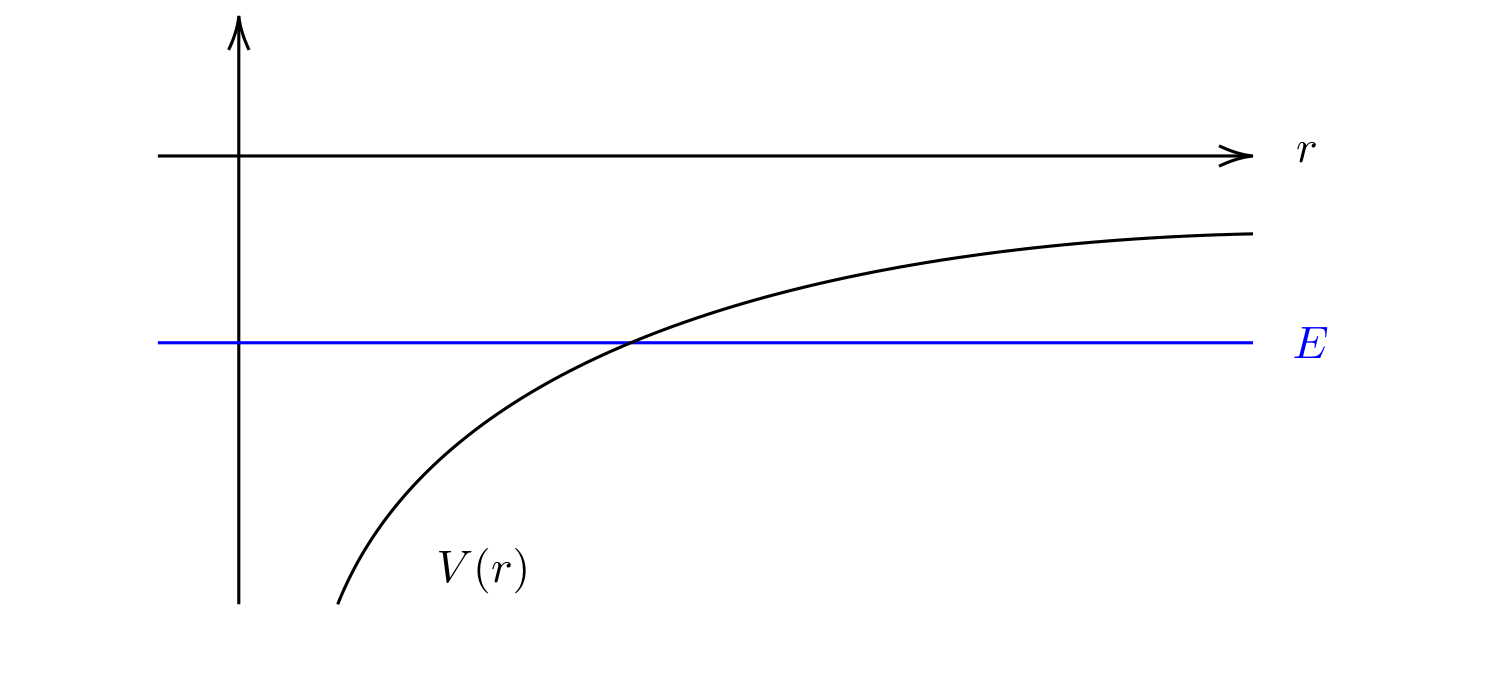
\includegraphics[width=0.66\textwidth]{figures/fig_p65_a.png}
\end{center}
% [图：原书 p.64，图内仅有数学符号标注]

% [原文 p.65]
对 \(E<0\)，记
\[
  B_E=\{\text{能量为 } E \text{ 的定态}\}.
\]
我们的目标是找出使能量本征空间 \(B_E\) 非平凡的那些允许的束缚态能量 \(E\)。

由于角动量 \(\hat J_i\) 与 \(\hat H\) 对易，它们实际上作用在空间 \(B_E\) 上。于是 \(B_E\) 构成三维旋转 \(\mathrm{SO}(3)\) 的一个表示。这对 \(B_E\) 施加了重要的约束，但不足以确定 \(E\)，因为这些对称性的生成元不含哈密顿量 \(\hat H\)。

另一方面，平方反比律的开普勒问题具有增强的对称性
\[
  \mathrm{SO}(3)\longrightarrow \mathrm{SO}(4)
\]
其生成元含有哈密顿量。这将使我们能算出束缚态能谱。下面讨论这一增强的对称性。

\subsection{增强的对称性}

\subsubsection*{经典拉普拉斯–龙格–楞次向量}

考虑质量为 \(m\) 的粒子在势 \(V=-\frac{Z}{r}\) 中运动。经典哈密顿量为
\[
  H=\frac{p^2}{2m}-\frac{Z}{r}.
\]
在平方反比力的开普勒问题中，存在一个额外的守恒量，称为\emph{拉普拉斯–龙格–楞次向量}（Laplace–Runge–Lenz vector）。经典的拉普拉斯–龙格–楞次向量为
\[
  \vec A=\frac{\vec p\times\vec J}{mZ}-\frac{\vec r}{r}.
\]
\(\vec A=(A_1,A_2,A_3)\) 的经典守恒性来自泊松括号关系
\[
  \{H,A_k\}=0,\qquad k=1,2,3
\]
它们可以直接验证。这使我们能如下求解经典运动。考虑内积
\[
  \vec A\cdot\vec r=\frac{(\vec p\times\vec J)\cdot\vec r}{mZ}-r
  =\frac{(\vec r\times\vec p)\cdot\vec J}{mZ}-r=\frac{J^2}{mZ}-r.
\]
我们写 \(\vec A\cdot\vec r=Ar\cos\theta\)，其中 \(A\) 是 \(\vec A\) 的长度，\(\theta\) 是 \(\vec A\) 与 \(\vec r\) 的夹角。由于 \(A\) 与 \(J^2\) 都守恒，因而都是运动常数，我们得到
\[
  r=\frac{J^2}{mZ}\frac{1}{1+A\cos\theta}.
\]
这立刻说明经典开普勒问题中的轨道必是椭圆（\(A<1\)）、抛物线（\(A=1\)）或双曲线（\(A>1\)）。

% [原文 p.66]
经典地，直接计算给出如下泊松括号关系
\[
  \{A_k,A_j\}=-\frac{2}{mZ^2}\sum_{l}\epsilon_{kjl}A_lH.
\]
此外，我们有
\[
  \vec A\cdot\vec J=0
\]
\[
  A^2=\vec A\cdot\vec A=1+\frac{2H}{mZ^2}J^2.
\]
设经典能量为负，即 \(H<0\)。此时 \(A<1\)，轨道是椭圆。它们是束缚态的经典对应物。我们重新定义两个守恒向量
\[
  \vec I=\frac{\vec J+\sqrt{\dfrac{mZ^2}{2|H|}}\vec A}{2},
  \qquad
  \vec K=\frac{\vec J-\sqrt{\dfrac{mZ^2}{2|H|}}\vec A}{2}.
\]
它们满足如下泊松括号关系
\[
  \{I_i,I_j\}=\sum_l\epsilon_{ijl}I_l
\]
\[
  \{K_i,K_j\}=\sum_l\epsilon_{ijl}K_l
\]
\[
  \{I_i,K_j\}=0
\]
于是 \(\{\vec I,\vec K\}\) 构成李代数 \(\mathrm{so}(3)\oplus\mathrm{so}(3)\)，它与李代数 \(\mathrm{so}(4)\) 相同。由于 \(\vec I,\vec K\) 守恒（它们与 \(H\) 的泊松括号为零），我们断定经典开普勒问题具有增强的 \(\mathrm{SO}(4)\) 对称性。

\subsubsection*{量子拉普拉斯–龙格–楞次向量}

现在把上面的讨论推广到量子情形。定义量子拉普拉斯–龙格–楞次向量为
\[
  \hat A=\frac{1}{2mZ}\left(\hat p\times\hat J-\hat J\times\hat p\right)-\frac{\vec r}{r}.
\]
在量子情形
\[
  \hat p\times\hat J\ne-\hat J\times\hat p
\]
因为 \(\hat p\) 与 \(\hat J\) 的分量不对易。按分量写，我们有
\[
  \begin{cases}
    \hat A_1=\dfrac{1}{2mZ}\left[\left(\hat p_2\hat J_3-\hat p_3\hat J_2\right)
      -\left(\hat J_2\hat p_3-\hat J_3\hat p_2\right)\right]-\dfrac{\hat x_1}{r}\\[10pt]
    \hat A_2=\dfrac{1}{2mZ}\left[\left(\hat p_3\hat J_1-\hat p_1\hat J_3\right)
      -\left(\hat J_3\hat p_1-\hat J_1\hat p_3\right)\right]-\dfrac{\hat x_2}{r}\\[10pt]
    \hat A_3=\dfrac{1}{2mZ}\left[\left(\hat p_1\hat J_2-\hat p_2\hat J_1\right)
      -\left(\hat J_1\hat p_2-\hat J_2\hat p_1\right)\right]-\dfrac{\hat x_3}{r}
  \end{cases}
\]
利用对易关系 \([\hat J_k,\hat p_j]=i\hbar\sum_m\epsilon_{kjm}\hat p_m\)，我们得到
\[
  \hat J\times\hat p=-\hat p\times\hat J+2i\hbar\hat p.
\]

% [原文 p.67]
因此我们可以等价地写
\[
  \hat A=\frac{1}{mZ}\left(\hat p\times\hat J-i\hbar\hat p\right)-\frac{\vec r}{r}.
\]
我们还有
\[
  \hat A\cdot\hat J=\hat J\cdot\hat A=0
\]
\[
  \hat A\cdot\hat A=1+\frac{2\hat H}{mZ^2}\left(\hat J\cdot\hat J+\hbar^2\right).
\]
最后这个量子关系与经典关系相差一个量子修正 \(\hbar^2\)。

在量子情形，我们有如下对易关系（见练习。详细陈述可参看 [32]）
\[
  \begin{aligned}
    [\hat H,\hat A_i]&=[\hat H,\hat J_i]=0\\
    [\hat A_k,\hat A_j]&=-i\hbar\frac{2}{mZ^2}\sum_l\epsilon_{kjl}\hat J_l\hat H\\
    [\hat J_k,\hat A_j]&=i\hbar\sum_l\epsilon_{kjl}\hat A_l\\
    [\hat J_k,\hat J_j]&=i\hbar\sum_l\epsilon_{kjl}\hat J_l
  \end{aligned}
\]
由于 \(\hat A,\hat J\) 与 \(\hat H\) 对易，它们保持本征空间 \(B_E\)（\(E<0\)）
\[
  \hat A_i,\hat J_i:B_E\longrightarrow B_E.
\]
限制到这个子空间 \(B_E\) 上，我们有
\[
  [\hat A_k,\hat A_j]=-i\hbar\frac{2}{mZ^2}\sum_l\epsilon_{kjl}E\hat J_l.
\]
现在可以做与经典情形相同的构造，重新定义
\[
  \hat I=\frac{\hat J+\sqrt{\dfrac{mZ^2}{2|E|}}\hat A}{2},
  \qquad
  \hat K=\frac{\hat J-\sqrt{\dfrac{mZ^2}{2|E|}}\hat A}{2}
  \qquad \text{于子空间 } B_E \text{ 上}.
\]
它们的对易关系同样服从李代数 \(\mathrm{so}(3)\oplus\mathrm{so}(3)\)
\[
  [\hat I_j,\hat I_m]=i\hbar\sum_l\epsilon_{jml}\hat I_l
\]
\[
  [\hat K_j,\hat K_m]=i\hbar\sum_l\epsilon_{jml}\hat K_l
\]
\[
  [\hat I_j,\hat K_m]=0
\]
于是我们得到量子的 \(\mathrm{so}(4)\) 对称性。相应的卡西米尔元满足
\[
  \hat I\cdot\hat I=\hat K\cdot\hat K=\frac{mZ^2}{8|E|}-\frac{\hbar^2}{4}
  \qquad \text{于子空间 } B_E \text{ 上}.
\]
正是这个关系使我们能算出量子开普勒问题的束缚态能量。

% [原文 p.68]
\subsection{\texorpdfstring{\(\mathrm{so}(3)\)}{so(3)} 的表示}

我们回顾李代数 \(\mathrm{so}(3)\) 的表示的一些基本事实
\[
  \mathrm{so}(3)=\{A:3\times3 \text{ 实矩阵}\mid A^T=-A\}.
\]
这个李代数是三维的，一组基为
\[
  t_1=\begin{pmatrix}0&0&0\\ 0&0&-1\\ 0&1&0\end{pmatrix},\quad
  t_2=\begin{pmatrix}0&0&1\\ 0&0&0\\ -1&0&0\end{pmatrix},\quad
  t_3=\begin{pmatrix}0&-1&0\\ 1&0&0\\ 0&0&0\end{pmatrix}.
\]
它们的对易关系是
\[
  [t_i,t_j]=\sum_k\epsilon_{ijk}t_k.
\]
为研究表示，方便的做法是重新定义如下复化基
\[
  \begin{cases}
    L_+:=it_1-t_2\\
    L_-:=it_1+t_2\\
    L_3:=it_3
  \end{cases}
\]
它们满足对易关系
\[
  [L_3,L_+]=L_+
\]
\[
  [L_3,L_-]=-L_-
\]
\[
  [L_+,L_-]=2L_3
\]
此外，\(L_3\) 是厄米的 \(L_3=L_3^*\)，而 \(L_+,L_-\) 互为厄米伴随 \(L_+^*=L_-\)。

\(\mathrm{so}(3)\) 的一个表示是一个向量空间 \(V\) 连同李代数同态
\[
  \rho:\mathrm{so}(3)\longrightarrow \mathrm{gl}(V).
\]
我们关心有限维复表示。\(\mathrm{so}(3)\) 的不可约复表示已有分类：对每个非负的半整数 \(l=0,\frac{1}{2},1,\frac{3}{2},\cdots\)，恰存在一个不可约表示 \(V_l\) 的同构类，且 \(\dim_\C V_l=2l+1\)。

记 \(\rho_l:\mathrm{so}(3)\to\mathrm{gl}(V_l)\) 为相应的表示。于是在每个 \(V_l\) 上，元素 \(L_3\) 可对角化为
\[
  \rho_l(L_3)=
  \begin{pmatrix}
    -l & & & & & & \\
     & -l+1 & & & & & \\
     & & -l+2 & & & & \\
     & & & \ddots & & & \\
     & & & & l-2 & & \\
     & & & & & l-1 & \\
     & & & & & & l
  \end{pmatrix}.
\]

% [原文 p.69]
对易关系
\[
  [L_3,L_\pm]=\pm L_\pm
\]
说明 \(L_+\)（\(L_-\)）的作用会把 \(L_3\) 的本征值升高（降低）一。因此在表示空间 \(V_l\) 上，\(L_3,L_\pm\) 的作用形如
\begin{center}
  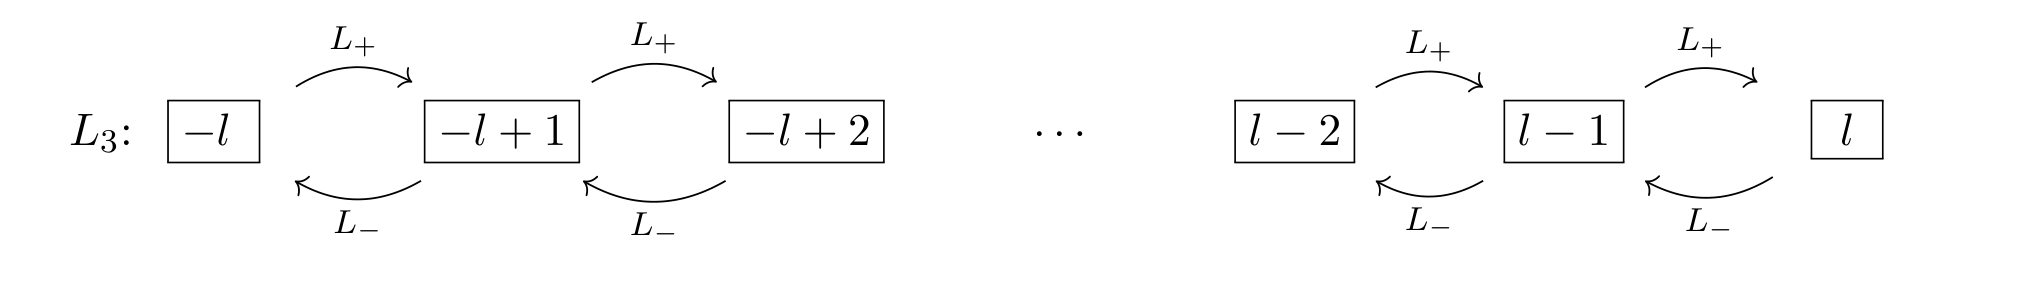
\includegraphics[width=0.98\textwidth]{figures/fig_p70_a.png}
\end{center}
% [图：原书 p.69，图内仅有数学符号标注]

区分这些表示的另一个办法是考虑卡西米尔元
\[
  \hat C=t_1^2+t_2^2+t_3^2=-L_3^2-\frac{1}{2}\left(L_+L_-+L_-L_+\right).
\]
卡西米尔元 \(\hat C\) 与所有 \(t_i\) 对易，因此在不可约表示上作用时成为常数。关键结果是：在不可约表示 \(V_l\) 上
\[
  \rho_l(\hat C)=-l(l+1).
\]
我们可以把上面的讨论推广到李代数 \(\mathrm{so}(4)=\mathrm{so}(3)\oplus\mathrm{so}(3)\) 的表示。那里有限维不可约表示按
\[
  V_k\otimes V_l,\qquad k,l=0,\frac{1}{2},1,\frac{3}{2},\cdots
\]
分类。一个 \(\mathrm{so}(3)\) 通过表示 \(\rho_k\) 作用在 \(V_k\) 因子上，而在 \(V_l\) 因子上作用为恒等。另一个 \(\mathrm{so}(3)\) 通过表示 \(\rho_l\) 作用在 \(V_l\) 因子上，而在 \(V_k\) 因子上作用为恒等。对应这两个 \(\mathrm{so}(3)\)，有两个卡西米尔元 \(\hat C_1,\hat C_2\)。在表示 \(V_k\otimes V_l\) 上，我们有
\[
  \hat C_1=-k(k+1),\qquad \hat C_2=-l(l+1)
  \qquad \text{于 } V_k\otimes V_l \text{ 上}.
\]

\subsection{能谱}

现在我们用 \(\mathrm{so}(3)\) 表示论分析量子开普勒问题。考虑哈密顿算子 \(\hat H\) 能量为 \(E<0\) 的本征空间 \(B_E\)。这对应束缚态。一般谱理论说明 \(B_E\) 是有限维的。

我们有算子
\[
  \hat I_i,\hat K_i:B_E\longrightarrow B_E
\]
作用在 \(B_E\) 上。于是 \(B_E\) 构成李代数 \(\mathrm{so}(4)=\mathrm{so}(3)\oplus\mathrm{so}(3)\) 的一个复表示。
\[
  [\hat I_j,\hat I_m]=i\hbar\sum_l\epsilon_{jml}\hat I_l
\]
\[
  [\hat K_j,\hat K_m]=i\hbar\sum_l\epsilon_{jml}\hat K_l
\]
\[
  [\hat I_j,\hat K_m]=0
\]

% [原文 p.70]
与 §1.11.3 的约定比较，\(\{I_i\}\) 这个 \(\mathrm{so}(3)\) 副本的卡西米尔元 \(\hat C_1\) 与 \(\{K_i\}\) 这个 \(\mathrm{so}(3)\) 副本的卡西米尔元 \(\hat C_2\) 为
\[
  \hat C_1=-\frac{\hat I^2}{\hbar^2},\qquad
  \hat C_2=-\frac{\hat K^2}{\hbar^2}.
\]
\(B_E\) 上的代数关系
\[
  \hat I\cdot\hat I=\hat K\cdot\hat K=\frac{mZ^2}{8|E|}-\frac{\hbar^2}{4}
\]
蕴含在 \(B_E\) 上 \(\hat C_1=\hat C_2\)。于是 \(B_E\) 由若干个 \(V_k\otimes V_k\) 组成（对某个 \(k\)）。此时
\[
  \hat C_1=\hat C_2=-k(k+1)
  \qquad\Longrightarrow\qquad
  |E|=\frac{mZ^2}{8\left(k+\frac{1}{2}\right)^2\hbar^2}.
\]
令 \(n=2k+1\)，它是正整数。于是可能的束缚态能量为
\[
  E_n=-\frac{mZ^2}{2\hbar^2n^2},\qquad n=1,2,\cdots.
\]
（经进一步分析可知）每个 \(E_n\) 确实出现在离散谱中，且每个 \(V_k\otimes V_k\) 恰好出现一次
\[
  B_{E_n}=V_{\frac{n-1}{2}}\otimes V_{\frac{n-1}{2}}.
\]
特别地，\(E_n\) 本征态空间的维数为
\[
  \dim B_{E_n}=\left(\dim V_{\frac{n-1}{2}}\right)^2=n^2.
\]

\subsection{氢原子}

氢原子由三维空间中的一个质子与一个电子组成。它可以看成一个两体量子力学问题。

记 \(\{\vec x_p,\vec p_p\}\) 为质子的位置与动量，\(\{\vec x_e,\vec p_e\}\) 为电子的位置与动量。相应的量子算子满足正则对易关系
\[
  \begin{aligned}
    \left[(\hat x_p)_i,(\hat p_p)_j\right]&=i\hbar\delta_{ij}\\
    \left[(\hat x_e)_i,(\hat p_e)_j\right]&=i\hbar\delta_{ij}\\
    \left[\hat x_p \text{ 或 } \hat p_p,\ \hat x_e \text{ 或 } \hat p_e\right]&=0.
  \end{aligned}
\]
氢原子的量子哈密顿量为
\[
  \hat H=\frac{\hat p_p^2}{2m_p}+\frac{\hat p_e^2}{2m_e}+V(|\vec x_e-\vec x_p|)
\]
其中 \(m_p\) 是质子质量，\(m_e\) 是电子质量。\(V\) 是中心库仑势
\[
  V(r)=-\frac{e^2}{r},
\]

% [原文 p.71]
其中 \(e\) 是基本电荷。

我们可以引入质心坐标来简化这个问题。确切地说，定义质心的位置与动量算子为
\[
  \hat x_c=\frac{m_e\hat x_e+m_p\hat x_p}{m_e+m_p},\qquad
  \hat p_c=\hat p_p+\hat p_e.
\]
定义相对位置与相对动量算子为
\[
  \hat x_R=\hat x_e-\hat x_p,\qquad
  \hat p_R=\frac{m_p\hat p_e-m_e\hat p_p}{m_e+m_p}.
\]
可以验证它们仍满足正则对易关系
\[
  \begin{aligned}
    \left[(\hat x_c)_i,(\hat p_c)_j\right]&=i\hbar\delta_{ij}\\
    \left[(\hat x_R)_i,(\hat p_R)_j\right]&=i\hbar\delta_{ij}\\
    \left[\hat x_c \text{ 或 } \hat p_c,\ \hat x_R \text{ 或 } \hat p_R\right]&=0.
  \end{aligned}
\]
于是我们可以改用 \(\hat x_c,\hat p_c,\hat x_R,\hat p_R\) 来处理。哈密顿算子此时变为
\[
  \hat H=\frac{\hat p_c^2}{2M_c}+\frac{\hat p_R^2}{2M_R}+V(|\vec x_R|)
\]
其中
\[
  M_c=m_e+m_p,\qquad M_R=\frac{m_em_p}{m_e+m_p}.
\]
利用分离变量，可以求解定态薛定谔方程
\[
  \psi(x_c,x_R)=\psi_c(x_c)\psi_R(x_R)
\]
其中 \(\psi_c(x_c)\) 与 \(\psi_R(x_R)\) 分别满足
\[
  \frac{\hat p_c^2}{2M_c}\psi_c=E_c\psi_c
\]
\[
  \left(\frac{\hat p_R^2}{2M_R}+V(|\vec x_R|)\right)\psi_R=E_R\psi_R.
\]
总能量为
\[
  E=E_c+E_R.
\]
关于 \(\psi_c\) 的方程说明质心像质量为 \(M_c\) 的自由粒子一样运动。关于 \(\psi_R\) 的方程说明质子与电子之间的相对运动是一个量子开普勒问题。由 §1.11.4 的结果，束缚态的能量 \(E_R\) 是量子化的
\[
  E_{R,n}=-\frac{M_Re^4}{2\hbar^2n^2},\qquad n=1,2,\cdots.
\]
能量为 \(E_{R,n}\) 的束缚态个数为 \(n^2\)。

这个公式恰好解释了原子氢的发射光谱：它出现在电子从一个较高的能态跃迁（或跳跃）到较低能态之时。观测到的谱线与上面两能级之间的能量差相符。

\takeaway{量子开普勒问题用库仑势描述。角动量构成 \(\mathrm{SO}(3)\) 对称性，但不足以决定能谱；拉普拉斯–龙格–楞次向量给出增强的 \(\mathrm{SO}(4)\) 对称性。在负能本征空间上，两个 \(\mathrm{so}(3)\) 副本的卡西米尔元相等，由此得到 \(E_n=-\frac{mZ^2}{2\hbar^2n^2}\) 与 \(n^2\) 重简并。}

% [原文 p.72]
\section{量子纠缠}

本节借助一个简单的有限维量子系统讨论量子纠缠这一重要现象。这个系统称为二维自旋系统，其状态空间是二维希尔伯特空间
\[
  V=\C^2.
\]

\subsection{自旋系统}

\subsubsection*{泡利矩阵与自旋算子}

考虑 \(V=\C^2\) 上的厄米算子 \(A\)。设
\[
  A=\begin{pmatrix}a&b\\ c&d\end{pmatrix},\qquad a,b,c,d\in\C.
\]
自伴条件 \(A=A^\dagger\) 要求
\[
  \begin{pmatrix}a&b\\ c&d\end{pmatrix}=\begin{pmatrix}\bar a&\bar c\\ \bar b&\bar d\end{pmatrix}
  \qquad\Longrightarrow\qquad
  a,d\in\R,\quad b=\bar c.
\]
因此 \(A\) 可以唯一地写成
\[
  A=\alpha_0I_2+\alpha_1\sigma_x+\alpha_2\sigma_y+\alpha_3\sigma_z,
  \qquad \alpha_i\in\R.
\]
这里 \(I_2=\begin{pmatrix}1&0\\ 0&1\end{pmatrix}\) 是单位矩阵，而 \(\sigma_x,\sigma_y,\sigma_z\) 称为\emph{泡利矩阵}：
\[
  \sigma_x=\begin{pmatrix}0&1\\ 1&0\end{pmatrix},\quad
  \sigma_y=\begin{pmatrix}0&-i\\ i&0\end{pmatrix},\quad
  \sigma_z=\begin{pmatrix}1&0\\ 0&-1\end{pmatrix}.
\]
泡利矩阵 \(\sigma_x,\sigma_y,\sigma_z\) 的本征值都是 \(\pm1\)，并满足如下关系
\[
  \begin{cases}
    \sigma_x^2=\sigma_y^2=\sigma_z^2=I_2\\
    \sigma_x\sigma_y=i\sigma_z=-\sigma_y\sigma_x\\
    \sigma_y\sigma_z=i\sigma_x=-\sigma_z\sigma_y\\
    \sigma_z\sigma_x=i\sigma_y=-\sigma_x\sigma_z
  \end{cases}
\]
更一般地，我们可以构造沿任意方向的自旋算子。

\begin{definition}{1.12.1}
对单位向量 \(\vec n=(n_x,n_y,n_z)\)，定义沿 \(\vec n\) 方向的自旋算子
\[
  \sigma_{\vec n}:=\vec\sigma\cdot\vec n=n_x\sigma_x+n_y\sigma_y+n_z\sigma_z
\]
\end{definition}

\begin{center}
  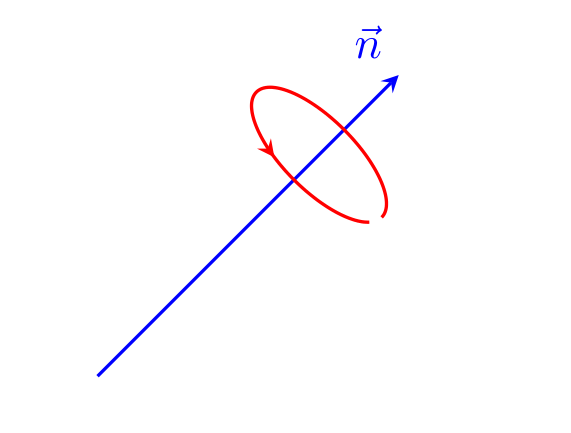
\includegraphics[width=0.26\textwidth]{figures/fig_p73_a.png}
\end{center}
% [图：原书 p.72，图内仅有数学符号标注]

% [原文 p.73]
\(\sigma_{\vec n}\) 的本征值为 \(\pm1\)，并满足
\[
  \sigma_{\vec n}^2=\left(n_x^2+n_y^2+n_z^2\right)I_2=I_2.
\]

\subsubsection*{自旋态}

\begin{center}
  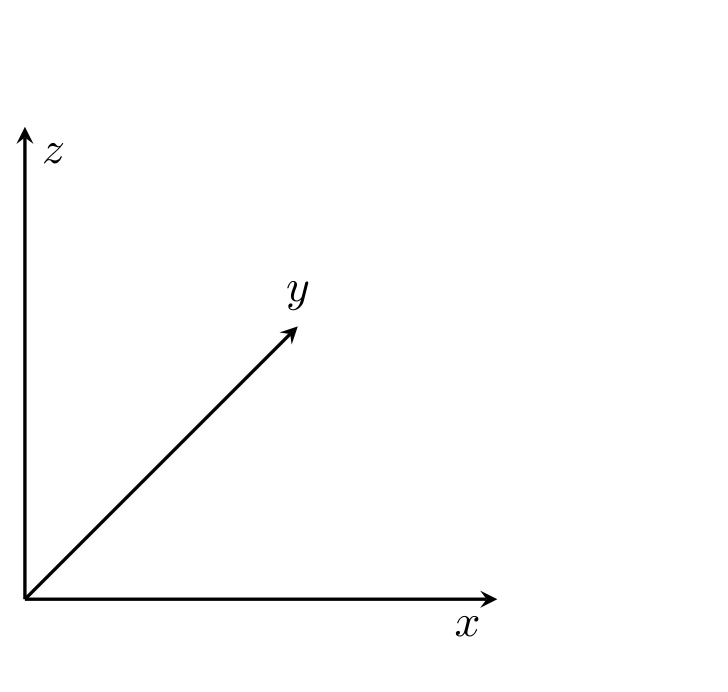
\includegraphics[width=0.30\textwidth]{figures/fig_p74_a.png}
\end{center}
% [图：原书 p.73，图内仅有数学符号标注]

让我们考虑自旋系统 \(V\) 中的一些标准基向量：

\begin{enumerate}[label=\arabic*.,leftmargin=2.2em,itemsep=2pt]
  \item \(\sigma_z\) 的本征向量：
  \[
    |u\rangle=\binom{1}{0},\qquad |d\rangle=\binom{0}{1}
  \]
  \[
    \sigma_z|u\rangle=|u\rangle,\qquad \sigma_z|d\rangle=-|d\rangle
  \]
  其中 \(u\) 表示“上”，意为自旋向上；\(d\) 表示“下”，意为自旋向下。

  \item \(\sigma_x\) 的本征向量：
  \[
    |r\rangle=\frac{1}{\sqrt2}\binom{1}{1},\qquad
    |l\rangle=\frac{1}{\sqrt2}\binom{1}{-1}
  \]
  \[
    \sigma_x|r\rangle=|r\rangle,\qquad \sigma_x|l\rangle=-|l\rangle
  \]
  其中 \(r\) 表示“右”，意为自旋向右；\(l\) 表示“左”，意为自旋向左。

  \item \(\sigma_y\) 的本征向量：
  \[
    |i\rangle=\frac{1}{\sqrt2}\binom{1}{i},\qquad
    |o\rangle=\frac{1}{\sqrt2}\binom{1}{-i}
  \]
  \[
    \sigma_y|i\rangle=|i\rangle,\qquad \sigma_y|o\rangle=-|o\rangle
  \]
  其中 \(i\) 表示“入”，意为自旋向内；\(o\) 表示“出”，意为自旋向外。
\end{enumerate}

这三组基都是正交归一的，它们之间的关系为
\[
  \begin{cases}
    |r\rangle=\frac{1}{\sqrt2}|u\rangle+\frac{1}{\sqrt2}|d\rangle\\[4pt]
    |l\rangle=\frac{1}{\sqrt2}|u\rangle-\frac{1}{\sqrt2}|d\rangle
  \end{cases}
  \qquad
  \begin{cases}
    |i\rangle=\frac{1}{\sqrt2}|u\rangle+\frac{i}{\sqrt2}|d\rangle\\[4pt]
    |o\rangle=\frac{1}{\sqrt2}|u\rangle-\frac{i}{\sqrt2}|d\rangle
  \end{cases}
\]
更一般地，沿单位向量 \(\vec n=(n_x,n_y,n_z)\) 自旋的态是 \(\sigma_{\vec n}\) 的本征向量。

% [原文 p.74]
\begin{example}{1.12.2}
考虑 \(\R^3\) 中的 \(\vec n=(\sin\theta,0,\cos\theta)\)。相应的自旋算子为
\[
  \sigma_{\vec n}=\sin\theta\cdot\sigma_x+\cos\theta\cdot\sigma_z
  =\begin{pmatrix}\cos\theta&\sin\theta\\ \sin\theta&-\cos\theta\end{pmatrix}.
\]
本征值 \(\lambda_1=1\) 与 \(\lambda_2=-1\) 对应的本征向量为
\[
  |\lambda_1\rangle=\binom{\cos\frac{\theta}{2}}{\sin\frac{\theta}{2}},\qquad
  |\lambda_2\rangle=\binom{-\sin\frac{\theta}{2}}{\cos\frac{\theta}{2}}.
\]
\begin{center}
  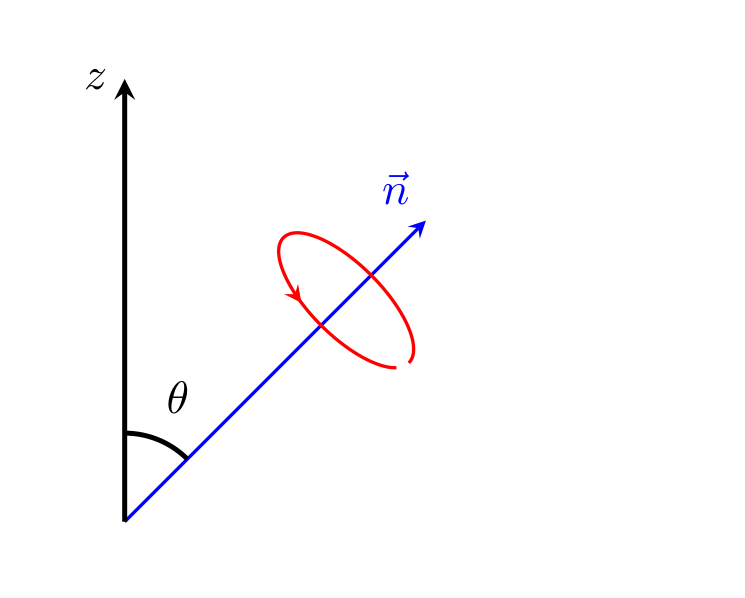
\includegraphics[width=0.34\textwidth]{figures/fig_p75_a.png}
\end{center}
% [图：原书 p.74，图内仅有数学符号标注]

考虑在归一态 \(|u\rangle\) 中测量算子 \(\sigma_{\vec n}\)。按测量的概率解释，测量结果可能是 \(\lambda_1\) 或 \(\lambda_2\)，相应的概率为
\[
  P(\lambda_1)=\left|\langle\lambda_1|u\rangle\right|^2=\cos^2(\theta/2)
\]
\[
  P(\lambda_2)=\left|\langle\lambda_2|u\rangle\right|^2=\sin^2(\theta/2)
\]
若计算算子 \(\sigma_{\vec n}\) 在态 \(|u\rangle\) 中的期望值（平均值）：
\[
  \langle u|\sigma_{\vec n}|u\rangle
  =\lambda_1\cos^2(\theta/2)+\lambda_2\sin^2(\theta/2)
  =\cos^2(\theta/2)-\sin^2(\theta/2)=\cos\theta.
\]
这个平均值反映了如下经典事实：\(\vec n\) 与 \(z\) 轴的夹角为 \(\theta\)。
\end{example}

\begin{example}{1.12.3}
对任意归一态 \(|\psi\rangle\in\C^2\)，存在单位向量 \(\vec n\) 使得
\[
  \langle\sigma_{\vec n}\rangle_\psi=1.
\]
\end{example}

\begin{proof}
设 \(|\psi\rangle\) 与 \(|\psi^\perp\rangle\) 构成 \(\C^2\) 的一组正交归一基。在这组基上定义算子
\[
  A:|\psi\rangle\mapsto|\psi\rangle,\qquad |\psi^\perp\rangle\mapsto-|\psi^\perp\rangle.
\]
\(A\) 是厄米的，且 \(\operatorname{Tr}(A)=0\)，因此它可以写成
\[
  A=n_x\sigma_x+n_y\sigma_y+n_z\sigma_z=\vec n\cdot\vec\sigma.
\]
由 \(A^2=I\) 可知 \(\vec n\) 是单位向量。并且
\[
  A|\psi\rangle=|\psi\rangle
  \qquad\Longrightarrow\qquad
  \langle\sigma_{\vec n}\rangle_\psi=\langle\psi|A|\psi\rangle=1
\]
\end{proof}

% [原文 p.75]
\subsection{纠缠态}

考虑由两个自旋粒子组成的复合系统。状态空间由张量积给出
\[
  \C^2\otimes\C^2.
\]
这个状态空间的一组基是
\[
  |uu\rangle=|u\rangle\otimes|u\rangle
\]
\[
  |ud\rangle=|u\rangle\otimes|d\rangle
\]
\[
  |du\rangle=|d\rangle\otimes|u\rangle
\]
\[
  |dd\rangle=|d\rangle\otimes|d\rangle
\]
在这组基下，\(\C^2\otimes\C^2\) 中的态 \(|\psi\rangle\) 可以表示为
\[
  |\psi\rangle=\sum_{\alpha,\beta\in\{u,d\}}c_{\alpha\beta}|\alpha\beta\rangle,
  \qquad c_{\alpha\beta}\in\C.
\]

\begin{definition}{1.12.4}
若 \(|\psi\rangle\in\C^2\otimes\C^2\) 可以写成
\[
  |\psi\rangle=|\phi\rangle\otimes|\chi\rangle
\]
则称它为\emph{积态}（product state）。不能表示成积态的态称为\emph{纠缠态}。
\end{definition}

\begin{example}{1.12.5}
量子态
\[
  |\psi\rangle=\frac{1}{2}|uu\rangle-\frac{1}{2}|ud\rangle
  +\frac{1}{2}|du\rangle-\frac{1}{2}|dd\rangle
\]
是积态。可以验证
\[
  |\psi\rangle=\left(\frac{1}{\sqrt2}|u\rangle+\frac{1}{\sqrt2}|d\rangle\right)
  \otimes\left(\frac{1}{\sqrt2}|u\rangle-\frac{1}{\sqrt2}|d\rangle\right)
  =|r\rangle\otimes|l\rangle.
\]
\end{example}

\begin{example}{1.12.6}
由
\[
  |s\rangle=\frac{1}{\sqrt2}\left(|ud\rangle-|du\rangle\right)
\]
定义的\emph{单态}（singlet state）是纠缠态。
\end{example}

\begin{proof}
设 \(|s\rangle=(\alpha_1|u\rangle+\alpha_2|d\rangle)\otimes(\beta_1|u\rangle+\beta_2|d\rangle)\)，展开得
\[
  \frac{1}{\sqrt2}\left(|ud\rangle-|du\rangle\right)
  =\alpha_1\beta_1|uu\rangle+\alpha_1\beta_2|ud\rangle
  +\alpha_2\beta_1|du\rangle+\alpha_2\beta_2|dd\rangle.
\]
比较系数：
\[
  \begin{cases}
    \alpha_1\beta_1=0\\[2pt]
    \alpha_1\beta_2=\dfrac{1}{\sqrt2}\\[6pt]
    \alpha_2\beta_1=-\dfrac{1}{\sqrt2}\\[6pt]
    \alpha_2\beta_2=0
  \end{cases}
\]
这导致矛盾，故 \(|s\rangle\) 是纠缠态。
\end{proof}

% [原文 p.76]
可以验证，\(|s\rangle\) 还可以表示为
\[
  |s\rangle=\frac{1}{\sqrt2}\left(|lr\rangle-|rl\rangle\right)
  =\frac{i}{\sqrt2}\left(|io\rangle-|oi\rangle\right).
\]

\subsection{EPR 佯谬}

现在我们考虑双自旋系统 \(\C^2\otimes\C^2\) 中的量子算子。我们把自旋算子延拓为
\[
  \sigma_\alpha^{(1)}:=\sigma_\alpha\otimes I_2,\qquad
  \sigma_\alpha^{(2)}:=I_2\otimes\sigma_\alpha,\qquad
  \alpha=x,y,z.
\]
它们在复合状态空间 \(\C^2\otimes\C^2\) 上的作用为
\[
  \sigma_\alpha^{(1)}\left(|\phi_1\rangle\otimes|\phi_2\rangle\right)
  =\left(\sigma_\alpha|\phi_1\rangle\right)\otimes|\phi_2\rangle
\]
\[
  \sigma_\alpha^{(2)}\left(|\phi_1\rangle\otimes|\phi_2\rangle\right)
  =|\phi_1\rangle\otimes\left(\sigma_\alpha|\phi_2\rangle\right)
\]
考虑在单态 \(|s\rangle\) 中测量其中一个分量的自旋。直接计算给出
\[
  \langle\sigma_x^{(1)}\rangle_s=\langle\sigma_y^{(1)}\rangle_s
  =\langle\sigma_z^{(1)}\rangle_s=0.
\]
因此对任意方向 \(\vec n\)：
\[
  \langle\sigma_{\vec n}^{(1)}\rangle_s=0.
\]
类似地
\[
  \langle\sigma_{\vec n}^{(2)}\rangle_s=0.
\]
这意味着，若我们只测量纠缠态 \(|s\rangle\) 中一个粒子的自旋，则任意方向上的测量期望值都为零！

\begin{center}
\begin{tikzpicture}[scale=0.95,>=Stealth]
  \node[circle,draw,thick,fill=blue!15,minimum size=1.1cm] (s1) at (0,0) {\small 1};
  \node[circle,draw,thick,fill=red!15,minimum size=1.1cm] (s2) at (4.6,0) {\small 2};
  \draw[<->,thick,red!65!black] (s1.east) -- node[above,text=black,font=\small]{纠缠态 $|s\rangle$} (s2.west);
  \node[text=blue!60!black,font=\small] at (0,1.15) {Alice};
  \node[text=red!70!black,font=\small] at (4.6,1.15) {Bob};
  \draw[->,blue!60!black] (0,0.95) -- (s1.north);
  \draw[->,red!70!black] (4.6,0.95) -- (s2.north);
\end{tikzpicture}
\end{center}
% [图：原书 p.76，本图按原文重绘，图内叙述文字已译为中文，人名为原文；原图无题注]

现在考虑把纠缠态 \(|s\rangle\) 中的两个自旋粒子分开到彼此相距很远的位置，让 Alice 与 Bob 分别在两边做测量。按量子力学的基本原理：

\begin{enumerate}[label=\arabic*.,leftmargin=2.2em,itemsep=2pt]
  \item 当 Alice 测量 \(\sigma_z^{(1)}\) 时，若测量结果为 \(+1\)（即 \(\sigma_z^{(1)}=+1\)），则由本征向量分解
  \[
    |s\rangle=\frac{1}{\sqrt2}\left(|ud\rangle-|du\rangle\right)
  \]
  可知量子态坍缩为 \(|ud\rangle\)。此时 Bob 的系统成为 \(|d\rangle\) 态，测 \(\sigma_z^{(2)}\) 将得到 \(-1\)。即
  \[
    \sigma_z^{(1)}=+1\qquad\Longrightarrow\qquad \sigma_z^{(2)}=-1
  \]

  类似地，若 Alice 测量 \(\sigma_z^{(1)}\) 得到 \(-1\)，则量子态坍缩为 \(|du\rangle\)，Bob 测 \(\sigma_z^{(2)}\) 将得到 \(+1\)。即
  \[
    \sigma_z^{(1)}=-1\qquad\Longrightarrow\qquad \sigma_z^{(2)}=+1
  \]

% [原文 p.77]
  \item 同样，由
  \[
    |s\rangle=\frac{1}{\sqrt2}\left(|lr\rangle-|rl\rangle\right)
  \]
  我们知道，若 Alice 测得 \(\sigma_x^{(1)}=\pm1\)，则 Bob 测得 \(\sigma_x^{(2)}=\mp1\)。
  \item 对 \(\sigma_y\) 的测量，我们也有 \(\sigma_y^{(1)}=\pm1\Rightarrow\sigma_y^{(2)}=\mp1\)。
\end{enumerate}

以上计算说明，无论纠缠态 \(|s\rangle\) 中的两个粒子相距多远，虽然测量单个粒子自旋的平均期望为零，但只要 Alice 做了自旋测量，Bob 在该方向上的自旋就立刻确定。这就是著名的爱因斯坦–波多尔斯基–罗森（EPR）佯谬：测量纠缠态中的一个粒子会瞬间影响另一个粒子。爱因斯坦称之为“幽灵般的超距作用”。

EPR 由此质疑量子力学的完备性。爱因斯坦主张隐变量理论，认为可能存在尚未发现的隐变量 \(\lambda\)，由它决定测量结果，从而避免任何不确定性或随机性。例如对态
\[
  \frac{1}{\sqrt2}|u\rangle+\frac{1}{\sqrt2}|d\rangle
\]
可能存在隐变量 \(\lambda\)，例如满足
\[
  \sigma_z(\lambda)=
  \begin{cases}
    +1 & \text{若 } 0\le\lambda\le\frac{1}{2}\\[4pt]
    -1 & \text{若 } \frac{1}{2}\le\lambda\le1
  \end{cases}
\]
若已知 \(\lambda\)，测量结果就被确定。测量的随机性源于我们对隐变量信息的无知。此外，隐变量还应满足定域性条件，即对一个粒子的测量不会瞬间影响另一个粒子。

\subsection{贝尔不等式}

1964 年，贝尔（Bell）提出了著名的贝尔不等式，为区分量子力学的预言与隐变量理论提供了具体可行的方案。此后，贝尔不等式的实验验证表明量子力学的预言是正确的，并且没有定域隐变量理论能解释量子纠缠的非经典关联。

% [原文 p.78]
\subsubsection*{量子力学计算}

考虑算子 \(\sigma_{n_1}^{(1)}\sigma_{n_2}^{(2)}=\sigma_{n_1}\otimes\sigma_{n_2}\) 在单态 \(|s\rangle\) 中的期望值：
\[
  P(\vec n_1,\vec n_2)=\langle s|\sigma_{n_1}^{(1)}\sigma_{n_2}^{(2)}|s\rangle.
\]
注意单态 \(|s\rangle\) 具有如下性质：
\[
  \begin{cases}
    \sigma_x^{(1)}|s\rangle=-\sigma_x^{(2)}|s\rangle\\[2pt]
    \sigma_y^{(1)}|s\rangle=-\sigma_y^{(2)}|s\rangle\\[2pt]
    \sigma_z^{(1)}|s\rangle=-\sigma_z^{(2)}|s\rangle
  \end{cases}
\]
因此对任意方向 \(\vec n\)：
\[
  \sigma_{\vec n}^{(2)}|s\rangle=-\sigma_{\vec n}^{(1)}|s\rangle
\]
于是得到
\[
  P(\vec n_1,\vec n_2)=\langle s|\sigma_{n_1}^{(1)}\sigma_{n_2}^{(2)}|s\rangle
  =-\langle s|\sigma_{n_1}^{(1)}\sigma_{n_1}^{(2)}|s\rangle
  =-(\vec n_1\cdot\vec n_2)\langle s|s\rangle=-(\vec n_1\cdot\vec n_2).
\]

\subsubsection*{隐变量理论计算}

假设存在隐变量 \(\lambda\)，满足
\[
  A(\vec n,\lambda)=\pm1,\qquad B(\vec n,\lambda)=\pm1
\]
并且（根据上面的实验测量结果）
\[
  A(\vec n,\lambda)=-B(\vec n,\lambda).
\]
假设在纠缠态 \(|s\rangle\) 中，隐变量服从概率分布 \(p(\lambda)\)，即满足
\[
  \sum_ip(\lambda_i)=1.
\]
按隐变量理论，测量 \(\sigma_{n_1}^{(1)}\sigma_{n_2}^{(2)}\) 的结果为
\[
  \tilde P(\vec n_1,\vec n_2)
  =\sum_ip(\lambda_i)A(\vec n_1,\lambda_i)B(\vec n_2,\lambda_i)
  =-\sum_ip(\lambda_i)A(\vec n_1,\lambda_i)A(\vec n_2,\lambda_i).
\]
现在考虑三个单位向量 \(\vec n_1,\vec n_2,\vec n_3\)，并计算
\[
  \begin{aligned}
    \tilde P(\vec n_1,\vec n_2)-\tilde P(\vec n_1,\vec n_3)
    &=-\sum_ip(\lambda_i)A(\vec n_1,\lambda_i)
      \left[A(\vec n_2,\lambda_i)-A(\vec n_3,\lambda_i)\right]\\
    &=-\sum_ip(\lambda_i)\left[1-A(\vec n_2,\lambda_i)A(\vec n_3,\lambda_i)\right]
      A(\vec n_1,\lambda_i)A(\vec n_2,\lambda_i).
  \end{aligned}
\]
这里我们用了 \(\left[A(\vec n,\lambda)\right]^2=1\)。因此
\[
  \left|\tilde P(\vec n_1,\vec n_2)-\tilde P(\vec n_1,\vec n_3)\right|
  \le\sum_ip(\lambda_i)\left[1-A(\vec n_2,\lambda_i)A(\vec n_3,\lambda_i)\right]
  =1+\tilde P(\vec n_2,\vec n_3).
\]
于是我们得到
\[
  \text{贝尔不等式：}\qquad
  \left|\tilde P(\vec n_1,\vec n_2)-\tilde P(\vec n_1,\vec n_3)\right|
  \le 1+\tilde P(\vec n_2,\vec n_3).
\]

% [原文 p.79]
\subsubsection*{量子力学与隐变量理论的比较}

取如下三个特定方向：
\[
  \vec n_1=(1,0,0),\qquad
  \vec n_2=(0,1,0),\qquad
  \vec n_3=\left(\frac{\sqrt2}{2},\frac{\sqrt2}{2},0\right)
\]

\begin{center}
  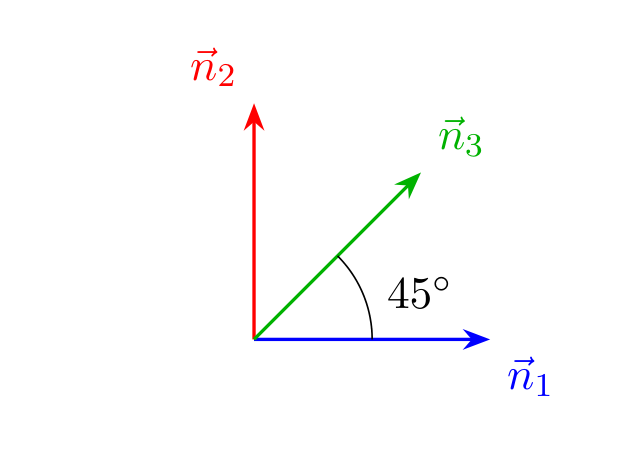
\includegraphics[width=0.34\textwidth]{figures/fig_p80_b.png}
\end{center}
% [图：原书 p.79，图内仅有数学符号标注]

量子力学预言：
\[
  P(\vec n_1,\vec n_2)=0,\qquad
  P(\vec n_1,\vec n_3)=-\frac{\sqrt2}{2},\qquad
  P(\vec n_2,\vec n_3)=-\frac{\sqrt2}{2}.
\]
于是
\[
  \left|P(\vec n_1,\vec n_3)-P(\vec n_1,\vec n_2)\right|
  =\left|-\frac{\sqrt2}{2}-0\right|=\frac{\sqrt2}{2}
\]
\[
  1+P(\vec n_2,\vec n_3)=1-\frac{\sqrt2}{2}
\]
由于 \(\frac{\sqrt2}{2}>1-\frac{\sqrt2}{2}\)，量子力学的预言会违反贝尔不等式。实验结果支持量子力学的预言。

\takeaway{二维自旋系统的态空间是 \(\C^2\)，泡利矩阵给出沿任意方向的自旋算子。两自旋的张量积空间里，态分为积态与纠缠态，单态是典型例子。测单态一侧即知另一侧，这是 EPR 佯谬；贝尔不等式随之与量子力学冲突，实验支持量子力学。}

\chapterreview{第 1 章从基本公设出发：态由希尔伯特空间中的向量描述，可观测量是自伴算子，测量遵循玻恩规则并使态向量坍缩，由此导出不确定原理。波函数把态实现为平方可积函数，位置与动量成为微分算子，薛定谔方程决定时间演化，定态对应能量本征态。随后用三个可解模型展示三类谱：自由粒子给出连续谱与波包，谐振子给出离散谱与阶梯算子，方势阱给出束缚态与散射态并存的混合谱。此后讨论一维散射与 \(S\) 矩阵、WKB 近似与半经典量子化规则，并借助角动量的 \(\mathrm{SO}(3)\) 对称性与增强的 \(\mathrm{SO}(4)\) 对称性解出量子开普勒问题与氢原子能谱。最后通过二维自旋系统与单态引出量子纠缠、EPR 悖论与贝尔不等式。}

% >>>CURSOR
